%*************************************************************
\chapter{Scribbler}\label{ch:scribbler} \index{Scribbler}
%*************************************************************

Die vergangenen Kapitel zeigen viele Beispiele, wie und mit welchen Hilfsmitteln Gruppenmeetings abgehalten werden können. Seien es traditionelle Medien wie Papier und Flip-Charts, oder elektronische Medien wie computerunterstützte Whiteboardsysteme - sie alle finden Einsatz in Designsessions und bieten verschiedenste Vor- und Nachteile.

\medskip Im folgenden wird \scribbler vorgestellt, ein elektronisches Interface, das die kollaborative Arbeit an virtuellen Artefakten unterstützt. Ähnlich wie die Autoren der bereits im ersten Kapitel beschriebenen Systeme, wurde mit \scribbler versucht, ein System zu kreieren, das die beiden Design-Arbeitswelten - geprägt durch traditionelle und elektronische Medien - mit einander verbindet und ihre Vorteile herausarbeitet. Im Gegensatz zu den bisherigen Ansätzen ist \scribbler ein elektronisches Skizziersystem, das ein barrierefreies Arbeiten ermöglicht.

\medskip Um dies zu zeigen, wird zuerst kurz die Ausgangssituation geschildert und danach die Anforderungen an ein kollaboratives Skizziersystem, die sich aus der Literaturrecherche ergeben haben, präsentiert. Danach wird die Vorgehensweise zur Erstellung des Prototyps erklärt, welche selbst einige Designmethoden aus \autoref{ch:designTheorie} beinhaltet. Anschließend folgt eine Präsentation der simplen Oberfläche von \scribbler und dessen Funktionsumfang mitsamt technischer Hintergründe. Schlussendlich werden die Anforderungen und Merkmale gegenübergestellt und die aus User-Tests gewonnenen Erkenntnisse beschrieben.

\section{Ausgangssituation \& Rahmenbedingungen} \label{sec:ausgangssituation} \index{Scribbler!Ausgangssituation}
Die Technisierung vieler Berufe führte dazu, dass gewisse Arbeitsgegenstände ein elektronisches Abbild bekamen. Im Gegensatz zu früher, fertigen Grafikdesigner heutzutage Präsentationszeichnungen oft an einem digitalen Medium an. Neuere Berufssparten wie Interfacedesign setzen die tagtägliche Arbeit mit digitalen Artefakten voraus. Wie schon in den vorigen Kapiteln erwähnt, ist (im Besonderen) Design eine kollaborative Tätigkeit, wofür sich Gruppen in Meetings treffen, um gemeinsam neue Lösungen zu erarbeiten. Ein bewährtes und wichtiges Instrument dazu sind Stifte zur Erstellung von Skizzen, um Gedanken auszudrücken.

Ein wesentlicher Bestandteil moderner Meetingräume ist ein zentraler Bildschirm oder Projektor, der als Präsentationsmedium eingesetzt wird. Zudem ist meistens eine Zeichenfläche vorhanden, wie z.B. Whiteboards oder Flip-Charts, um kollaborativ erarbeitete Ideen festzuhalten und neue Ideen zu explorieren.

\medskip Das Institut für Gestaltungs- und Wirkungsforschung an der TU Wien verfügt über so einen Meetingraum. Darin befinden sich mehrere Tische, die in der Mitte des Raumes zusammengestellt wurden und um die sich Sitzmöglichkeiten befinden. Neben einem Flip-Chart befindet sich ein {54\dq} großer Bildschirm in der Mitte einer Wand, auf den alle Meetingteilnehmer von ihren Sitzplätzen aus blicken können. Mit dem Screen ist ein Computer (Apple Mac Mini) verbunden, auf den Daten über ein drahtlos Netzwerk gespielt werden können. Eine zusätzliche drahtlose Tastatur und Maus ermöglichen eine bequeme Steuerung. Zusätzliche Peripherie kann an der Rückseite des Computers angeschlossen werden.

\medskip Das Kerngebiet des Instituts ist \ac{HCI}. Hier wird der Meetingraum oft dazu verwendet, Designs für interaktive Systeme, Applikationen oder Webinhalte zu erarbeiten. Erwartungsgemäß sind nur bereits umgesetzte Inhalte digital vorhanden. Diese Problematik macht den Einsatz der wichtigsten Designmethode - Skizzieren - auf dem Artefakt fast unmöglich. Das Ziel der vorliegenden Arbeit war es nun ein Tool zu entwickeln, das es ermöglicht, auf jegliche präsentierte Inhalte ob Webseiten, Programmoberflächen oder Bilder, >>kritzeln<< zu können. \scribbler soll so die Barriere zwischen der realen Welt und der digitalen Welt aufbrechen.

\section{Anforderungen an kollaborative Skizziersysteme} \label{sec:anforderungen} \index{Skizziersysteme!Anforderungen}
In den vorhergehenden Kapiteln wurde ein Überblick über das Verbesserungspotential vieler existierender Systeme gegeben. Wichtige literarische Größen auf diesem Gebiet, wie beispielsweise Lee, Olsen, Tang, Larsson, Johnson oder Prante, wiesen auf wesentliche Erkenntnisse hin, die ein solches System formen. Diese Erkenntnisse können vier großen Einflussfaktoren zugeordnet werden: \emph{Hardware}, \emph{Software}, \emph{Kollaboration} und \emph{Skizzieren} und bieten eine Art Checkliste für kollaborative Systeme. \autoref{fig:scribblerKollaborativesSkizziersystem} zeigt eine Aufstellung dieser Erkenntnisse, in Verbindung zu ihren Einflussfaktoren. 

\begin{figure}
	        {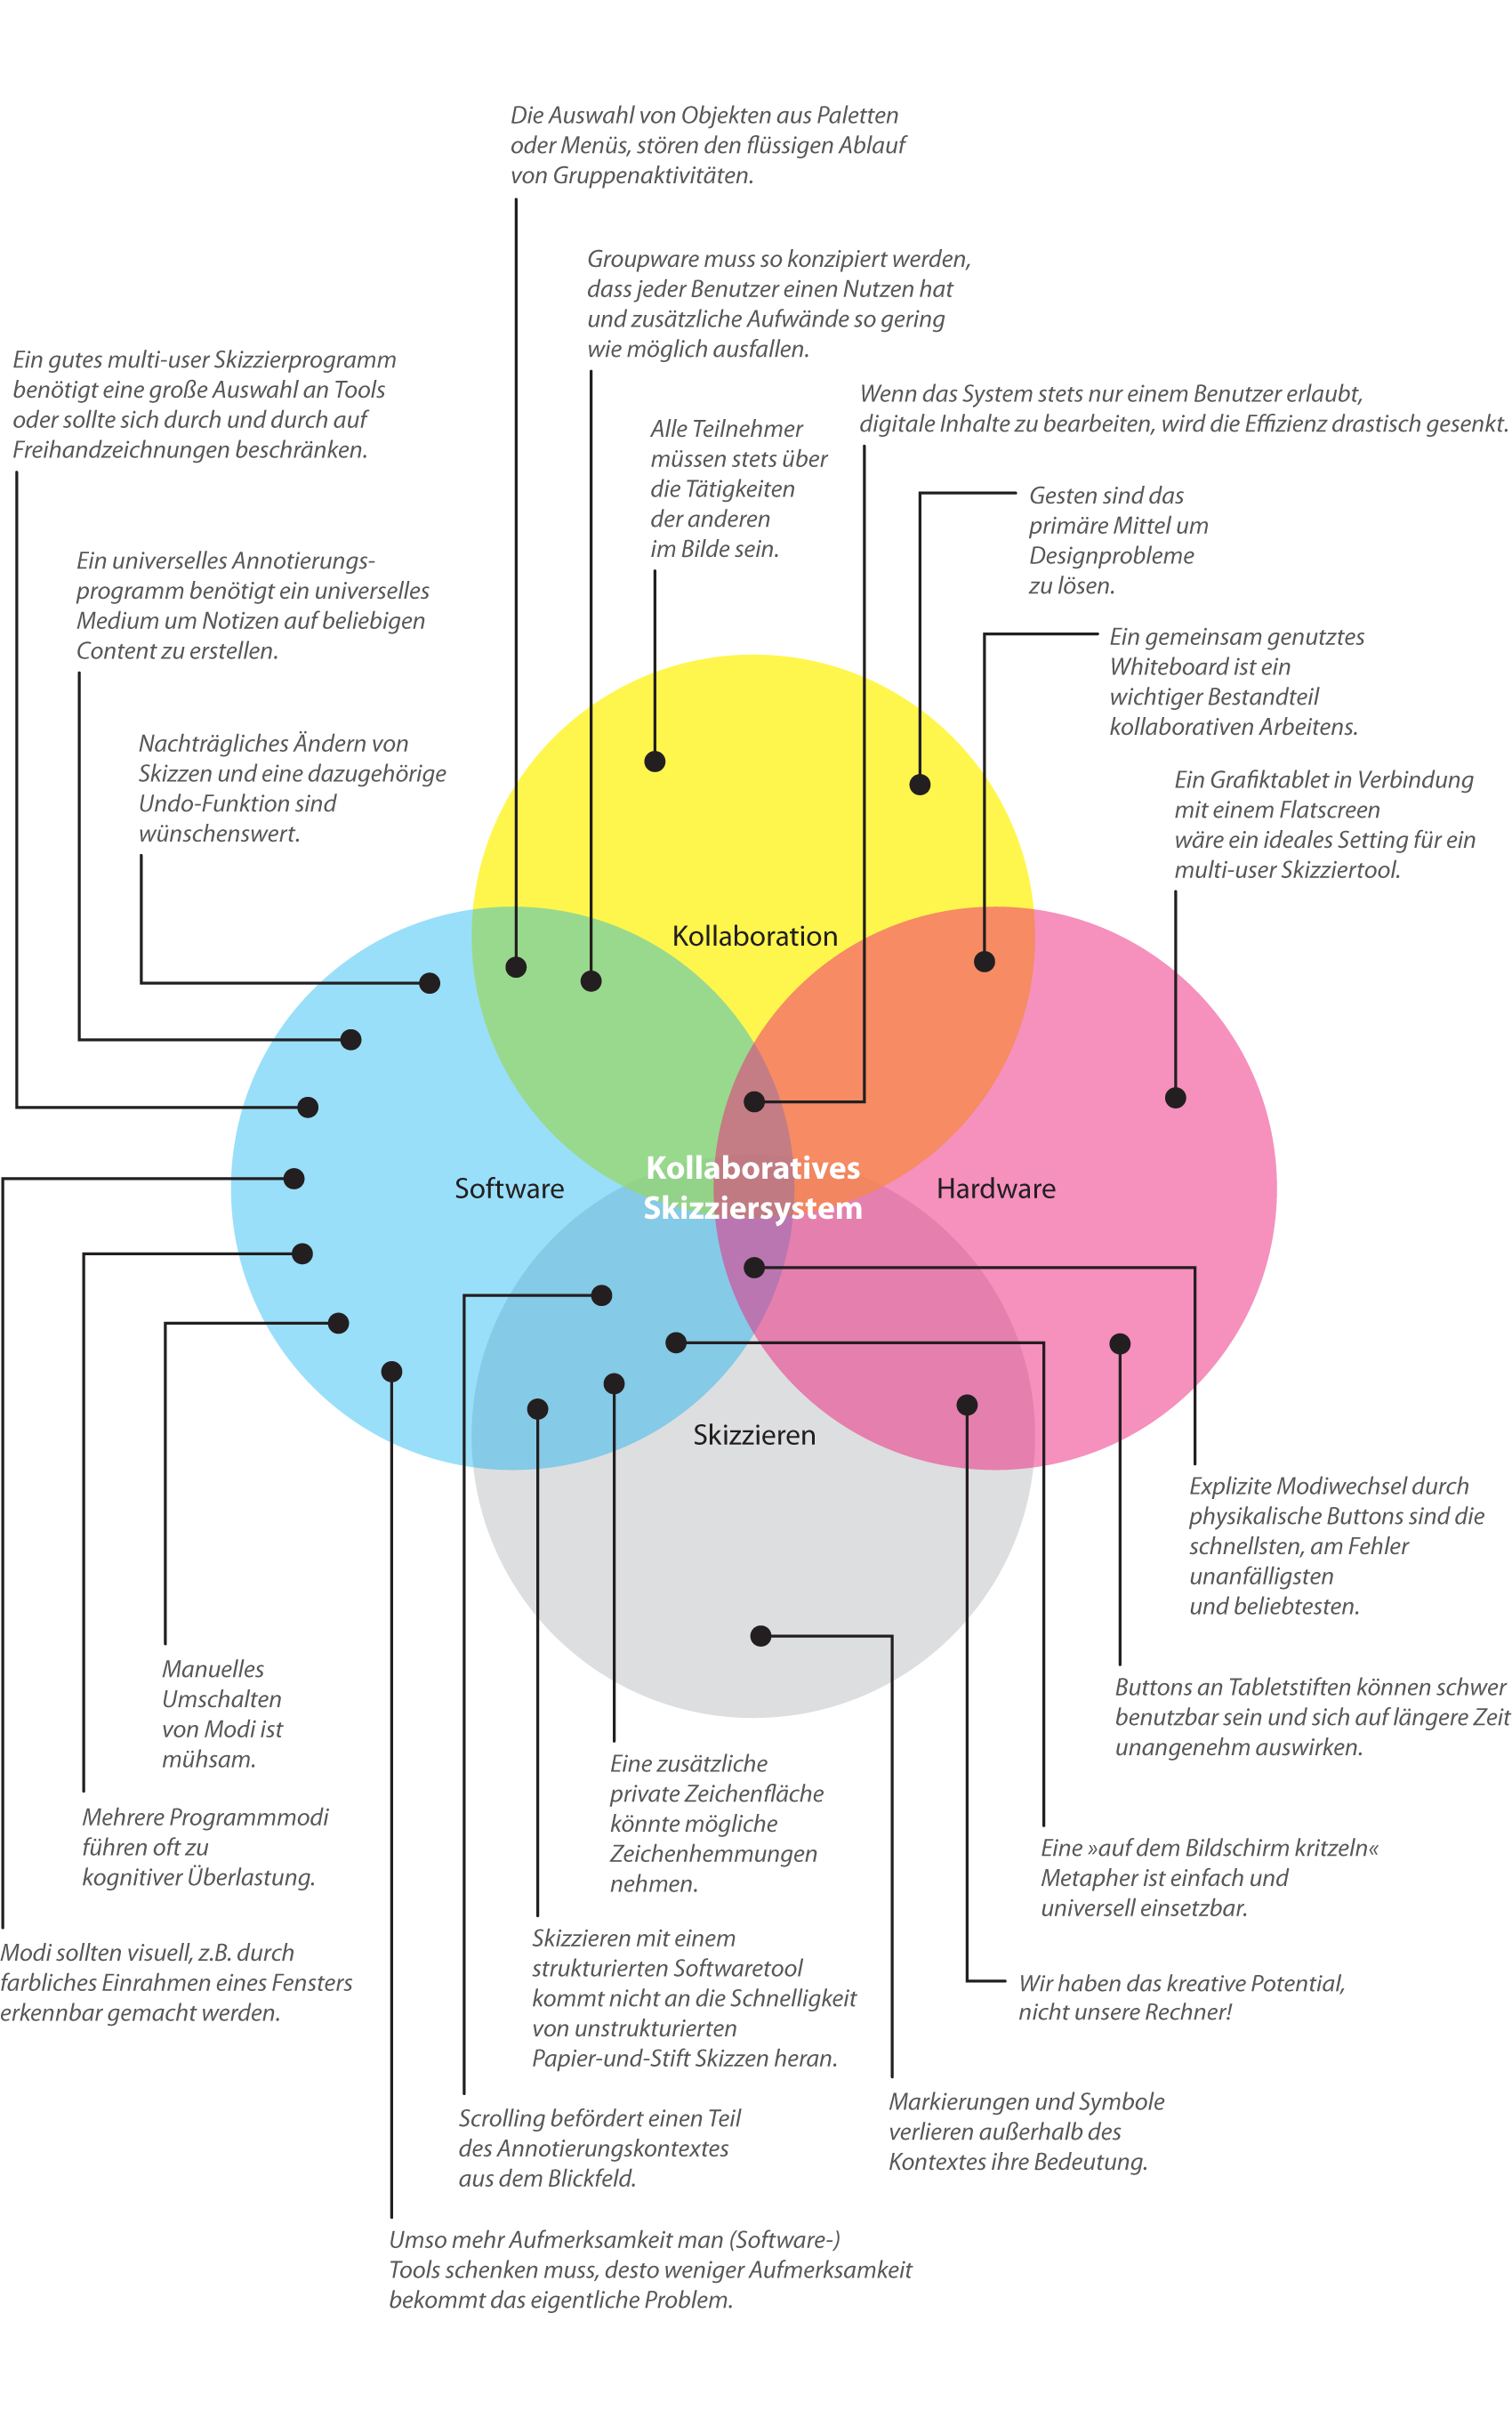
\includegraphics[bb=0cm 0cm 14.39cm 23.01cm]{gfx/scribblerKollaborativesSkizziersystem}}
		\caption[Anforderungen eines kollaborativen Skizzersystems]{Anforderungen eines kollaborativen Skizzersystems, bestehend aus den vier Einflussfaktoren: Hardware, Software, Kollaboration \& Skizzieren.}\label{fig:scribblerKollaborativesSkizziersystem}
\end{figure}

\subsubsection*{Hardware} Ein ideales Setting für ein kollaboratives Skizziertool wäre laut Lee ein Grafiktablet in Verbindung mit einem Flatscreen. Dies wäre die bestmögliche Annäherung an eine Technologie, die Stift und Papier ersetzen könnte. Sie würde ebenso zur Umsetzung eines Whiteboard Systems beitragen, was einen wichtigen Bestandteil kollaborativen Arbeitens ausmacht. Buttons an Tabletstiften können schwer benutzbar sein und sich auf längere Zeit unangenehm auswirken, deswegen sollte davon abgeraten werden diese mit Funktionen zu belegen. 

\subsubsection*{Software} Ein gutes multi-user Skizzierprogramm benötigt eine große Auswahl an Tools oder sollte sich ausschließlich auf Freihandzeichnungen beschränken. Welcher Ansatz besser funktioniert, müsse laut Lee ausprobiert werden. Je mehr Aufmerksamkeit ein Softwaretool erfordert, desto weniger Aufmerksamkeit kann jedoch dem eigentlichen Problem zukommen. Folglich sollte solch ein System so einfach wie möglich aufgebaut sein.

Die Verwendung mehrerer Programmmodi führt oftmals zu kognitiver Überlastung. Aus diesem Grund sollte der aktuelle Modus visuell, z.B. durch farbliches Einrahmen eines Fensters, erkennbar gemacht werden. Zudem ist das manuelle Umschalten von Modi mühsam. Explizite Modiwechsel durch physikalische Buttons sind dennoch die schnellsten, am Fehler unanfälligsten und beliebtesten. 

Will man ein universelles Annotierungstool schaffen, das über alle verwendeten Programme eines Benutzers funktioniert, benötigt man auch ein universelles Medium, um Notizen auf beliebigem Content zu erstellen. Außerdem wären das nachträgliche Ändern von Skizzen und eine dazugehörige Undo-Funktion wünschenswert.

\subsubsection*{Kollaboration} Gemeinsam genutzte Systeme müssen so konzipiert werden, dass jeder Teilnehmer einen Nutzen hat. Wenn das System nur einem Benutzer erlaubt digitale Inhalte zu bearbeiten, wird die Effizienz drastisch gesenkt. Zusätzliche Aufwände sollten so gering wie möglich ausfallen. Die Auswahl von Objekten aus Paletten oder Menüs, stören beispielsweise den flüssigen Ablauf von Gruppenaktivitäten. Die Teilnehmer der Kollaboration sollten ebenso stets über die Tätigkeiten der anderen im Bilde sein. Dabei spielen Gesten eine wichtige Rolle.

\subsubsection*{Skizzieren} Das Zeichnen mit einem strukturierten Softwaretool ersetzt nicht das Zeichnen von unstrukturierten Papier-und-Stift Skizzen. Eine >>auf dem Bildschirm kritzeln<< Metapher ist somit einfach und universell einsetzbar. Skizzen verlieren außerhalb des Kontextes ihre Bedeutung. Daher muss darauf geachtet werden, dass der Kontext stets bewahrt wird. Scrolling befördert z.B. einen Teil des Annotierungskontextes aus dem Blickfeld und benötigt somit zusätzliche Aufmerksamkeit bei der Umsetzung. Außerdem könnte eine zusätzliche, private Zeichenfläche mögliche Zeichenhemmungen von Teilnehmern nehmen. Schlussendlich haben die Benutzer das kreative Potential - ein Skizziersystem muss sich entsprechend adaptieren können.

\section{Vorgehensweise} \index{Scribbler!Vorgehensweise}
Aufgrund des Bedarfs nach einem elektronischen Skizziersystem wurde zuerst eine Suche nach vergleichbaren Systemen veranlasst. Eine Brainstorming-Sitzung diente dazu, verschiedene Begriffe zu sammeln und zu explorieren. Viele wissenschaftliche Datenbanken stellen eine Fülle an Literatur bereit, die wiederum Hinweise zu bestehenden kollaborativen Skizziertools liefert. Nach der Lektüre und Analyse der gesammelten Werke konnte ein vorläufiges Anforderungsprofil an solche Systeme erstellt werden.

Eine wichtige Designfrage stellte sich schon zu diesem Zeitpunkt: Welche Eingabetechnologie sollte für \scribbler eingesetzt werden? \autoref{fig:scribblerVorgehensweise} zeigt Aufzeichnungen zu der wohl wichtigsten hardwarespezifischen Frage. Nachträglich digitalisierte Skizzen, würden das System unabhängig von notwendigen Gerätschaften machen. Diese Voraussetzung käme der Flexibilität des Systems zu Gute. Jedoch ist es technisch aufwändig und fehleranfällig, gezeichnete Objekte nachträglich zu erkennen. Es müsste Mustererkennung zum Einsatz kommen, und das Ergebnis könnte unter Umständen nicht zufriedenstellend ausfallen. Würden Zeichnungen direkt auf digitalem Wege angefertigt, z.B. via Tablets, wäre die Flexibilität des Systems zwar eingeschränkt, das Ergebnis jedoch besser.

Im Hinblick auf \scribbler wurde zusammen mit dem Institut entschieden, auf die zweite Variante zu setzen, da Tablets bereits vorhanden waren und für einen ersten Prototypen ausreichen sollten.

\begin{figure}
	        {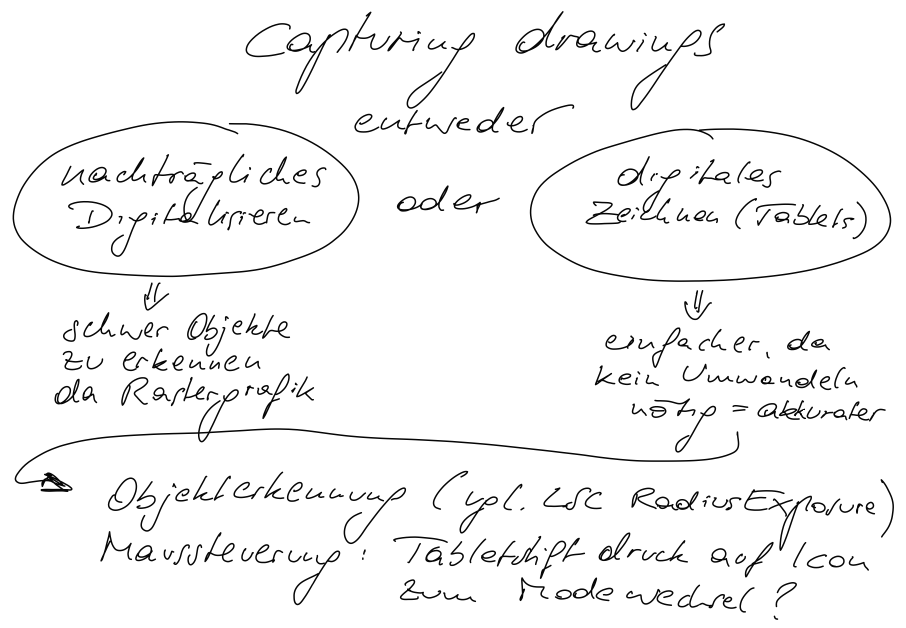
\includegraphics[width=1\linewidth]{gfx/scribblerVorgehensweise}}
		\caption[Aufzeichnung zur frühesten Designfrage]{Aufzeichnung zur frühesten Designfrage. Sollten Skizzen nachträglich digitalisiert werden oder sollte gleich auf digitales Zeichnen gesetzt werden?}\label{fig:scribblerVorgehensweise}
\end{figure}

Nachdem das grobe Konzept geklärt war, folgte der nächste Schritt, das Verstehen des eigentlichen Skizzierens. Es wurden dazu verschiedene Szenarios exploriert, um einen Einblick in die Praxis der Thematik zu erlangen. Anschließend wurden mehrere Mockups erstellt und das Skizzierverhalten von verschiedenen Probanden analysiert. Das Konzept konnte dadurch nach und nach verfeinert werden, doch aussagekräftigere Tests waren notwendig. Aus diesem Grund wurde bald mit der Anfertigung von Prototypen mit größerem Funktionsumfang begonnen. Die Mockups konnten auch nur Ein-Benutzer-Szenarios abdecken, weshalb schon bald mit der Implementierung begonnen wurde.

\bigskip \emph{Anmerkung: \graffito{\(\clubsuit\)} Zu diesem Zeitpunkt kam erstmals der Begriff >>Scribbler<< auf, der fortan als Codename für das Projekt benutzt wurde.}
\bigskip

Während der Implementierungsphase konnten Funktionalität und Verhalten des Systems durch interne Tests kontinuierlich verbessert werden. Mit Hilfe von potentiellen Nutzern wurde die finale Beta-Version von \scribbler einem Review unterzogen.

\medskip In den folgenden Punkten werden die angesprochenen und verwendeten Designmethoden (vgl. \autoref{sec:designmethoden}) beschrieben und mit Hilfe verschiedener Bilder veranschaulicht. Die Beschreibung des Designprozesses soll so angereichert und durch konkrete, praktische Beispiele verständlicher aufbereitet werden.

\subsection{Recherche}
Recherche ist nicht direkt den Designmethoden zuzuordnen, stellt aber trotzdem einen wichtigen Teil in der Entwicklung eines Produkts dar. Recherche ermöglicht Einsicht in den betehenden Markt und die aktuelle Forschung. Des weiteren wird ein Einblick in deren Funktionsweisen erlangt.

\medskip Durch die Literaturrecherche wurden einige vergleichbare Systeme gefunden, die jedoch die große Einschränkung hatten, dass Content und Input nicht miteinander verknüpft wurden. Es gibt zwar Annäherungen, jedoch bringen diese den Inhalt nur in eine statische Scheinbeziehung mit den Eingaben. Dies verdeutlichte die Notwendigkeit eines Skizziersystems wie \scribbler, das über die Grenzen des Instituts hinausgehen könnte.

Zusätzlich wies die Literatur bereits auf Probleme hin, die durch die notwendige Selektion eines Werkzeuges entstehen konnten (vgl. \pointref{sec:ModusProblem}).

\medskip Das Erlangen neuer Sichtweisen des Systems durch die ausgiebige Recherche resultierte schließlich im vorläufigen Anforderungsprofil.

\subsection{Skizzieren}
Alleiniges bzw. gemeinsames Skizzieren waren die wichtigsten Instrumente in der Anfangsphase von \scribbler. Skizzen ermöglichten die Veranschaulichung bzw. Generierung neuer Ideen und dienten somit auch als Diskussionsbasis. 

Aus der Literaturrecherche geht hervor, dass meistens ein Sitzungsteilnehmer als Schreiber fungiert und die wichtigsten, besprochenen Fakten in Stichwörtern und kurzen Sätzen zusammenfasst (vgl. \autoref{fig:scribblerVorgehensweise}). Skizzen wurden manchmal angefertigt um bestimmte Vorgehensweisen aus der Literatur zu illustrieren. Dies führte meist zu kollaborativen Arbeitsvorgängen, bei denen zusammen an einer Skizze gearbeitet wurde. 

\medskip Wie bereits erwähnt, wurden später Skizzen zu wichtigen Szenarios erstellt. Eine farbliche Kennzeichnung war dabei oft sehr hilfreich. Zudem konnten Zugehörigkeiten oder zeitliche Abläufe durch Hinzufügen von Nummerierungen leicht angedeutet werden (siehe \autoref{fig:scribblerSzenarien}).

\medskip Abschließend zeigt \autoref{fig:scribblerDetailSkizze} ein Beispiel einer detaillierten Skizze, die dazu verwendet wurde, technische Abläufe zu verstehen. Sie entstand im Laufe der Entwicklung, in der ständig neue Ideen aufkamen, die durch Skizzen innerhalb des Teams erforscht wurden.

\begin{figure}
	\begin{center}
	        {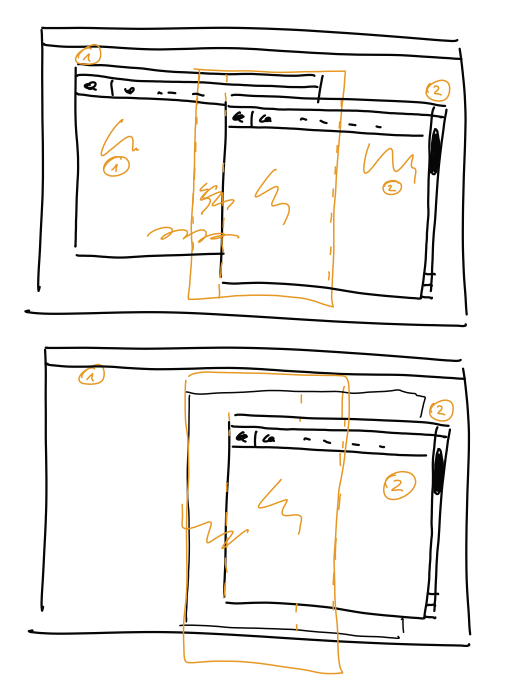
\includegraphics[width=0.8\linewidth]{gfx/scribblerSzenarien}}
		\caption[Skizzierte Szenarien in Scribbler]{Skizzierte Szenarien in Scribbler. Zugehörigkeiten wurden durch eine Nummerierung gekennzeichnet.}\label{fig:scribblerSzenarien}
	\end{center}
\end{figure}

\begin{figure}
	        {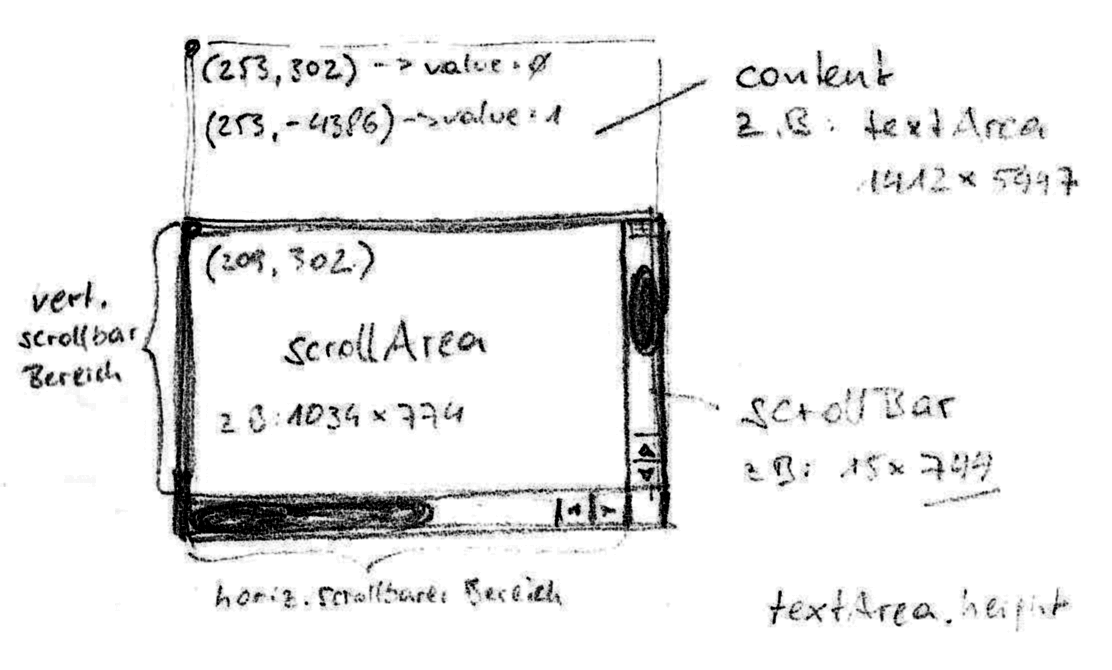
\includegraphics[width=1\linewidth]{gfx/scribblerDetailSkizze}}
		\caption[Detailskizze eines technischen Ablaufs]{Detaillierte Skizze eines technischen Ablaufs, um diesen besser zu verstehen.}\label{fig:scribblerDetailSkizze}
\end{figure}

\subsection{Prototyping}
Das Erarbeiten von Prototypen war keine leichte Aufgabe, da das Setting an sich, durch die verschiedenen Einflussfaktoren, kompliziert erschien. Dennoch konnten anfangs simple Prototypen, sogenannte Mockups angefertigt werden, um vorerst detailliertere Szenarios zu erstellen und später das Skizzierverhalten einiger Probanden zu beobachten. Mockups sind low-fidelity Prototypen, beispielsweise Papierprototypen. Dieser >>Wegwerfcharakter<< impliziert eine einfache Erstellung und rudimentäre Funktionalität, die für frühe Tests ausreicht.

\medskip \autoref{fig:scribblerMockups} zeigt ein Mockup, das im Wesentlichen nur aus einem Screenshot eines \acs{WIMP}-Systems bestand (in diesem Fall Mac OS X mit zwei offenen Programmfenstern) und in Verbindung mit einem Tablet PC benutzt wurde. Die konzipierten Szenarios, wurden durch den höheren Detailgrad konkreter, wodurch mehrere Funktionen im Voraus geplant werden konnten. Später wurden diese verwendet, um erste Tests durchzuführen. Der Prototyp beschränkte die Interaktionen der Benutzer auf das Skizzieren. So konnte beispielsweise festgestellt werden, welche Plätze zum Zeichnen gesucht werden, wie bestimmte Elemente markiert werden oder Zusammenhänge von Inhalten hergestellt werden.

\begin{figure}
	        {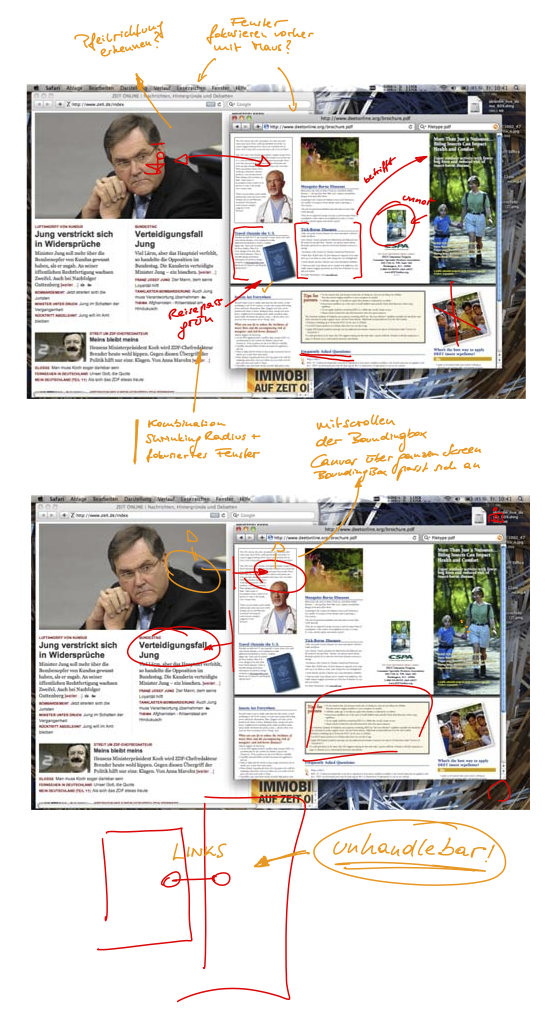
\includegraphics[width=1\linewidth]{gfx/scribblerMockups}}
		\caption[Mockups in Scribbler]{Simple Mockups, die durch Screenshots auf einem Tablet PC erstellt wurden.}\label{fig:scribblerMockups}
\end{figure}

\medskip Darauf folgende Prototypen als programmierte Versionen von \scribbler wurden ebenfalls getestet.

\subsection{(User) Testing}
Die erstellten Prototypen vor der Implementierung des Programms, ermöglichten die Testung eines kleinen Funktionsteils mit Usern. Wichtige Systemverhaltensweisen bzw. Interaktionen konnten aber nur durch zusätzliche Testdurchgänge während der Umsetzung, auf Verständlichkeit und Anklang geprüft werden.

\medskip Einen Vorteil stellte die geringe Vorbereitungszeit dar. Es mussten keine bestimmten Anweisungen oder Aufgaben gestellt werden. Zum einen sollte die reale Welt in Bezug auf das Skizzieren mit Papier und Stift nachgebildet werden. Zum anderen sollten keine aufwändigen Aufgaben notwendig sein, sodass Probanden einfach >>loskritzeln<< konnten.

\medskip Es bestand außerdem die Möglichkeit, \scribbler innerhalb einer Gruppe von fünf Personen zu testen, die an einem bestimmten Design arbeiteten und dazu den in \autoref{sec:ausgangssituation} beschriebenen Meetingraum vom Institut nutzten (siehe \autoref{fig:scribblerUserTest}).

\begin{figure}
	        {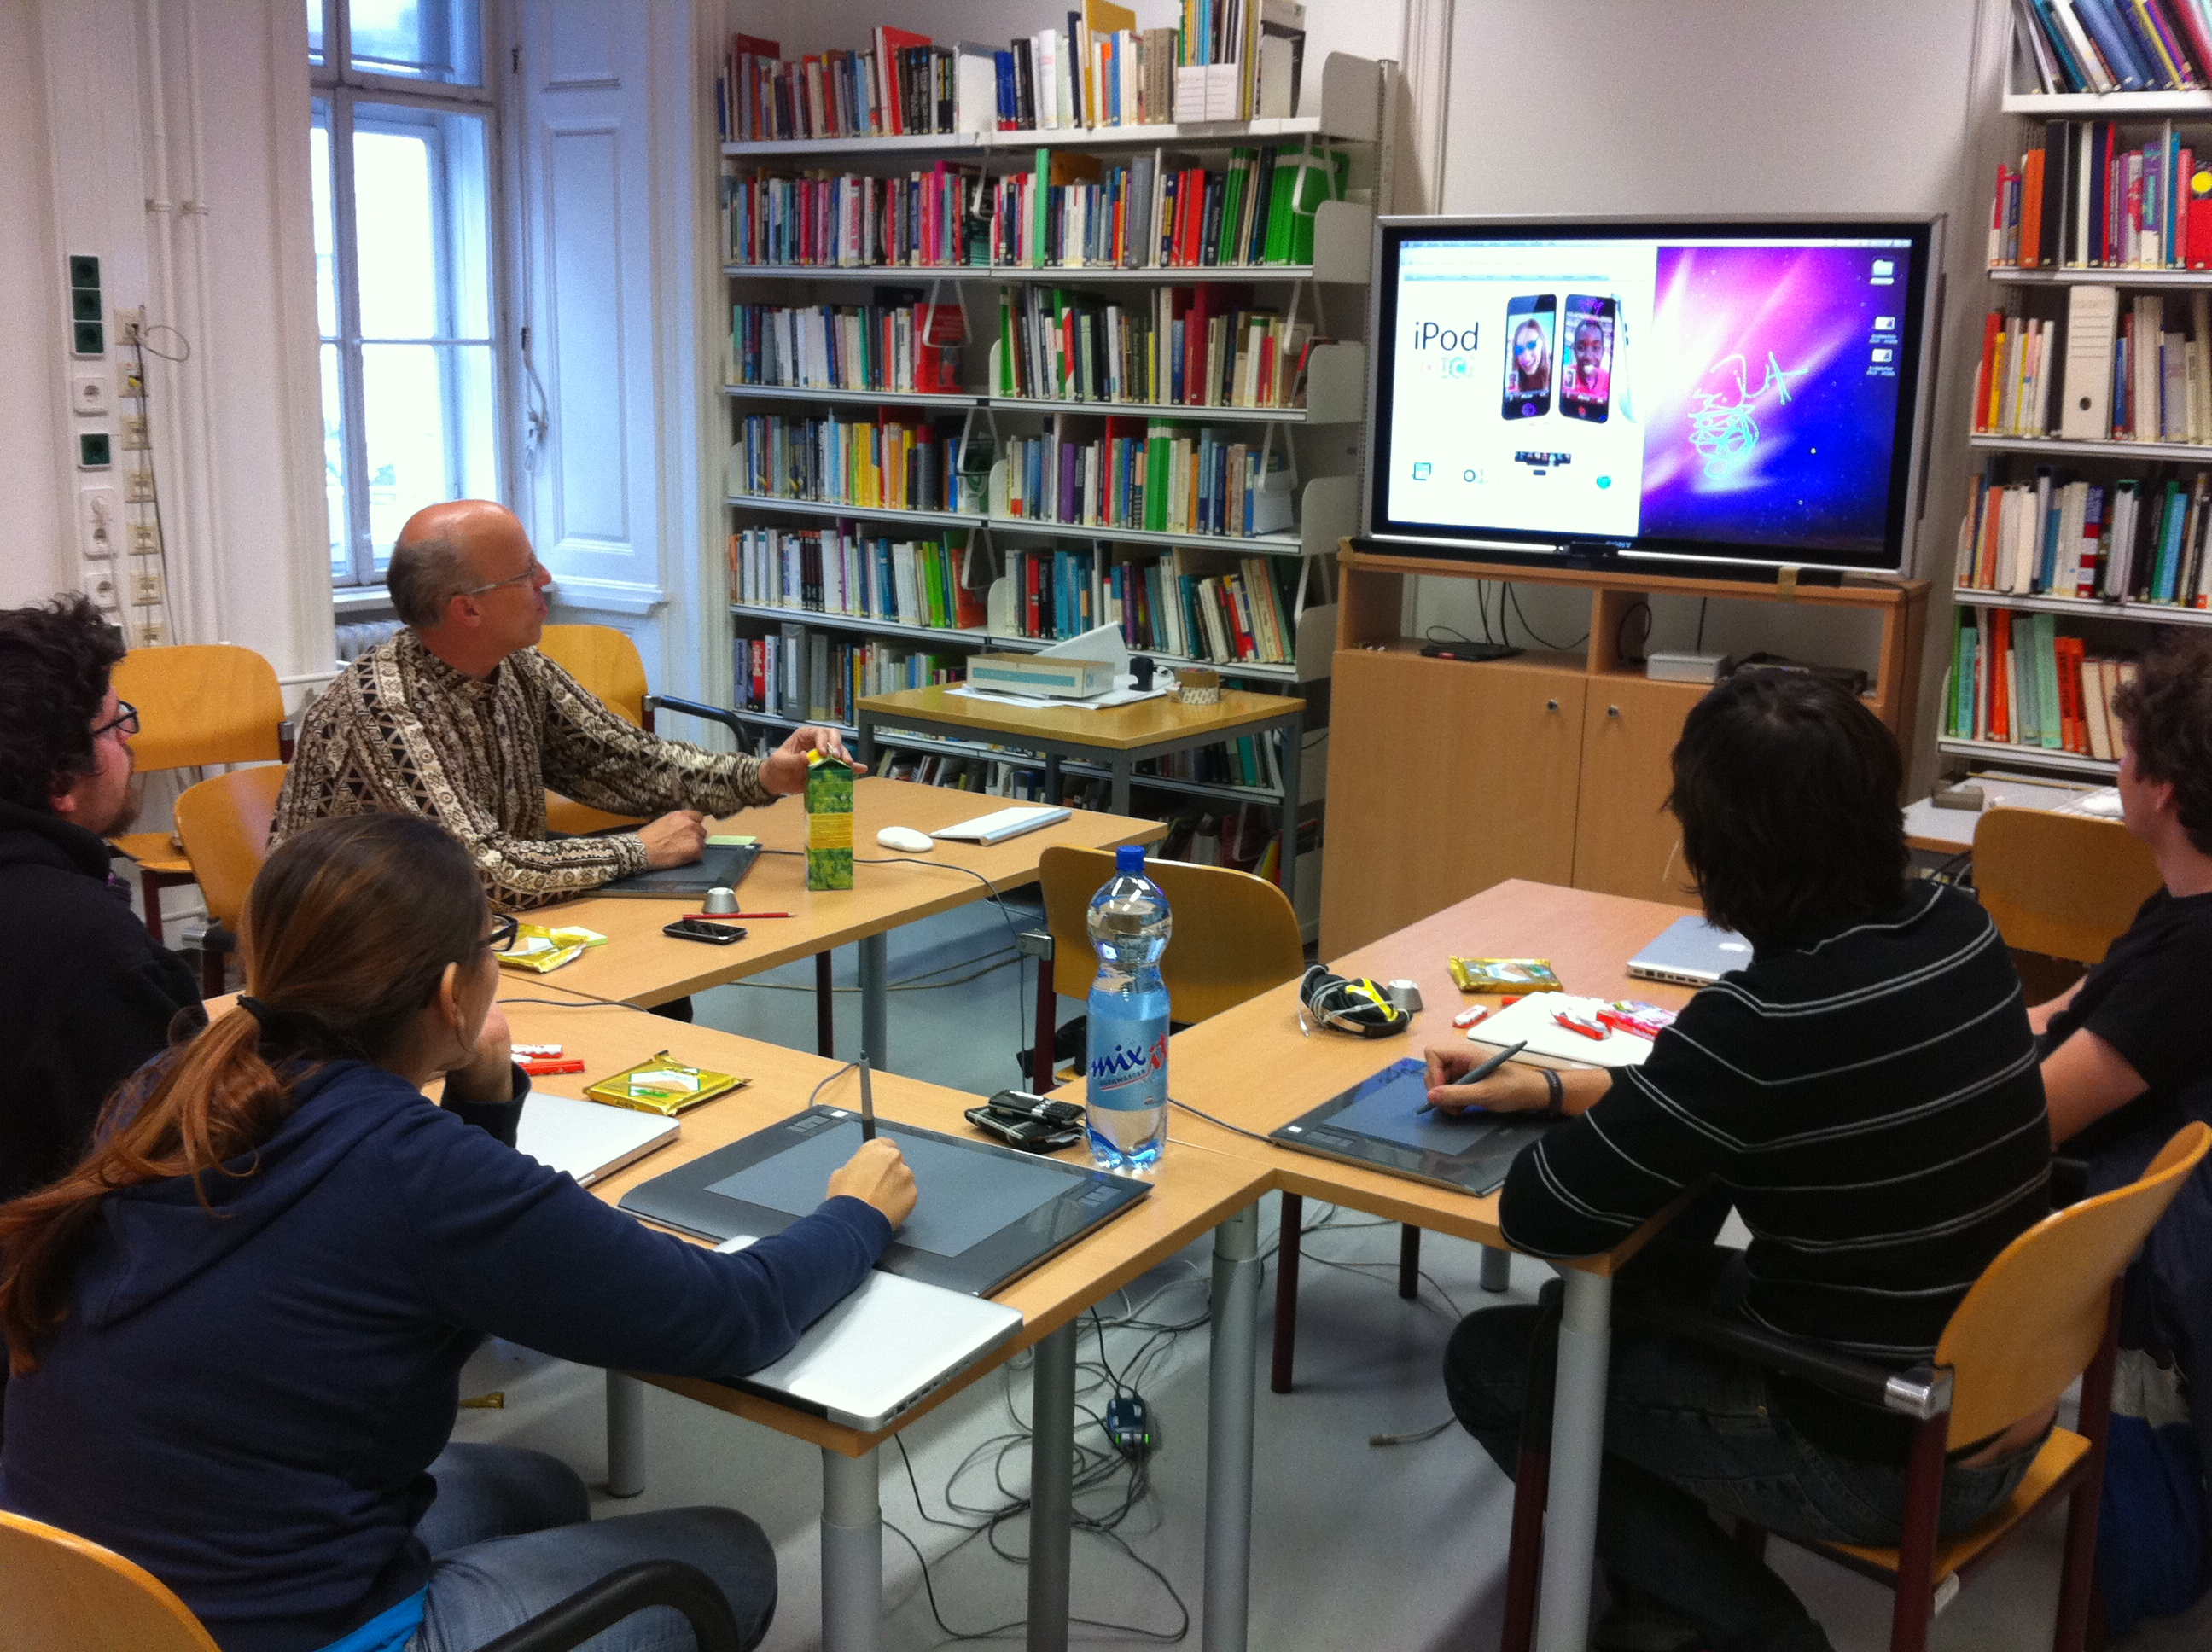
\includegraphics[width=1\linewidth]{gfx/scribblerUserTest}}
		\caption[Scribblertesting in einer Designsession]{Scribblertesting in einer Designsession. Fünf Personen überarbeiten mittels Scribbler ein Designvorschlag.}\label{fig:scribblerUserTest}
\end{figure}

\medskip Nach Fertigstellung der Betaversion konnte \scribbler zusätzlich am Beginners-Day\footnote{Der Beginners-Day ist eine Infoveranstaltung für alle Studienanfängerinnen und Studienanfänger in den Informatik-, Wirtschaftsinformatik- und Lehramtsstudien. \citep{TU:2010}} der TU Wien vorgeführt und mit vielen erstsemestrigen Studenten getestet werden. Abschließend konnten auch ausführliche Tests mit Designern durchgeführt werden, die in \autoref{sec:userReview} ausführlich beschrieben sind.

\section{Scribbler at a Glance} \index{Scribbler!at a Glance}
Durch die verschiedenen Designmethoden veränderte sich die Funktionalität von \scribbler öfters. Aus diesem Grund wird das Konzept erst in diesem Kapitel angeführt.

\medskip \scribbler ermöglicht neben der herkömmlichen Arbeit an einem Desktop (\acs{WIMP}) System, mittels Stiften auf jedes beliebige Programmfenster zu zeichnen. Das System läuft im Hintergrund und aktiviert sich bei Bedarf. Es unterscheidet dabei generell zwei Hauptmodi: den Zeichen- und den Mausmodus. In letzterem kann die Maus wie gewohnt zur Navigation zwischen Programmfenster eingesetzt werden. Die Verwendung eines Tabletstifts hingegen wechselt in den Zeichenmodus. Die Benutzer können so auf das momentan aktive Fenster einer Drittapplikation >>kritzeln<<. Da besonders geübte Tabletbenutzer die Stifte auch als Ersatz für die Maus verwenden, ermöglicht \scribbler auch das explizite Wechseln der beiden Modi durch Drücken einer Tablettaste.

\medskip Da beim Skizzieren natürlich auch Fehler auftreten können, bietet \scribbler eine >>Undo<< bzw. >>Redo<< Funktion. Versehentliche Aktionen können so rückgängig gemacht oder wiederhergestellt werden. Zudem können einzelne Striche gelöscht bzw. >>ausradiert<< oder der gesamte Zeichenbereich geleert werden.

\medskip Diese Grundfunktionalität soll vor allem Designer die Möglichkeit bieten, bestehende Arbeiten und Designs zu besprechen, Anmerkungen in direkter Verbindung zu digitalen Artefakten zu verfassen und kontextbezogene Erweiterungen zu zeichnen. Weil natürlich nicht immer schon vorhandene Designs vorliegen, bietet \scribbler aber auch eine Whiteboard Funktion. Hierbei wird eine weiße Fläche über den gesamten Bildschirm eingeblendet, auf dem Benutzer Raum zum freien Skizzieren bekommen.

\medskip Um erarbeitete Skizzen zu speichern, besitzt \scribbler eine Screenshot Funktion. Nur durch Speichern eines Bildes, kann aus unserer Sicht der Kontext zu den Zeichnungen bewahrt werden. Eine Unterbrechung, jedoch nicht Beendigung von \scribbler, erfolgt durch eine integrierte Standby Funktion.

\medskip Die folgenden Punkte sollen nun nähere Informationen zur Hardware, dem grafischen User Interface und dem logischen Programmaufbau geben. 

\subsection{Hardware} \label{ssec:hardware} \index{Scribbler!Hardware}
\scribbler benötigt ein relativ komplexes Hardware-Setting. Für die Ausgabe wird ein großes Display oder ein Beamer benutzt, während es für die Eingabe erforderlich ist, dass jeder Benutzer über ein Tablet mit Stift verfügt. Diese Tablets und das Ausgabegerät werden mit einem Rechner verbunden, auf dem das Apple Betriebssystem OS X 10.6 >>Snow Leopard<< läuft. Ältere Versionen von OS X werden von \scribbler nicht unterstützt. Für ein optimales Nutzungserlebnis sollte der Computer über eine gute Rechenleistung verfügen. Bei der Umsetzung des Prototypen fiel die Entscheidung auf die Nutzung von Tablets aus der Modellreihe Intuos3 von Wacom. Diese Geräte verfügen über jeweils vier Buttons an beiden Seiten neben der Zeichenoberfläche, die mit verschiedenen Funktionen belegt werden können. Über diese Tasten können die folgenden Aktionen durchgeführt werden:

\begin{itemize}
	\item \emph{Wechsel des Interaktionsmodus für den Tabletstift}\\
	Ermöglicht das Umschalten von Zeichen- in den Mausmodus und umgekehrt. (Dies betrifft nur den Tabletstift, die Maus selbst ist immer im Mausmodus und kann nicht zum Zeichnen verwendet werden)
	\item \emph{Whiteboard}\\
	Blendet eine weiße Fläche über den gesamten Screen ein oder aus. Auf dieser kann ebenfalls gezeichnet werden.
	\item \emph{Zurücksetzen}\\
	Löscht alle Zeichnungen des momentan aktiven Fensters.
	\item \emph{Sichern}\\
	Erstellt einen Schnappschuss des Bildschirm samt den Zeichnungen des aktiven Fensters und legt diesen in einer Datei am Schreibtisch ab.
\end{itemize}

\begin{figure}
	\begin{center}
        {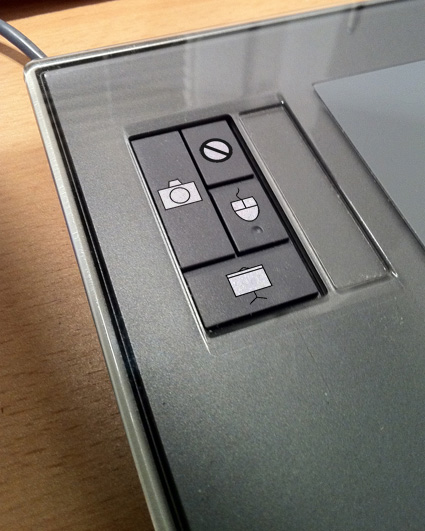
\includegraphics[width=0.8\linewidth]{gfx/scribblerTabletTasten}}
		\caption[Tablet Tastenbelegung]{Die Anordnung der \scribbler Funktionen auf den Tasten des Tablets. Der Fotoapparat links oben erstellt ein Bildschirmfoto, das Verbotszeichen auf der rechten, oberen Taste löscht alle Zeichnungen des aktiven Fensters, die Maus auf der genoppten, mittleren Taste wechselt den Interaktionsmodus und das Whiteboard auf der unteren Taste blendet selbiges ein oder aus.}\label{fig:scribblerTabletTasten}
	\end{center}
\end{figure}

\autoref{fig:scribblerTabletTasten} zeigt die Anordnung der Buttons auf den Tablets. Die mittlere Taste ist mit einer Noppe versehen und bietet dadurch ein haptisches Feedback. Dadurch kann der Button ertastet werden ohne dass ein Hinsehen von Nöten ist. Sinnvollerweise sollte diese Taste mit der wichtigsten Funktion belegt werden. In \scribbler ist dies der Wechsel des Interaktionsmodus, denn dieser ermöglicht, den vollen Interaktionsumfang mit nur einem Eingabegerät (dem Stift) zu nutzen. Die anderen beiden wichtigen Funktionen, sprich das Bildschirmfoto und das Whiteboard, liegen auf den zwei großen Tasten links oben und unten. Das Zurücksetzen aller Zeichnungen wird relativ selten gebraucht und liegt daher auf der kleinen Taste rechts oben. Damit Benutzer diese Anordnung nicht auswendig lernen müssen, wurden bei den Tests entsprechende Icons an den Tasten angebracht. Auf der rechten Seite der Zeichenoberfläche des Tablets sind die selben Tasten spiegelverkehrt angebracht, damit auch Linkshänder \scribbler optimal verwenden können.

\medskip Neue Wacom Tablets werden üblicherweise mit nur einem Stift ausgeliefert. In den Testsettings wurden jedem Benutzer mehrere Stifte zur Verfügung gestellt. Diese verfügen alle über eine Hardware-ID und können dadurch von \scribbler eindeutig identifiziert werden. So ist es möglich, jedem Stift eine eigene Farbe zuzuordnen. \autoref{fig:scribblerColors} zeigt vier Stifte mit unterschiedlichen Farben. Um dies klar zu machen, wurde jeder Stift mit einem entsprechend gefärbten Sticker versehen. Der Wechsel zwischen Farben war dadurch so intuitiv wie das Wechseln zwischen zwei Buntstiften.

\begin{figure}
        {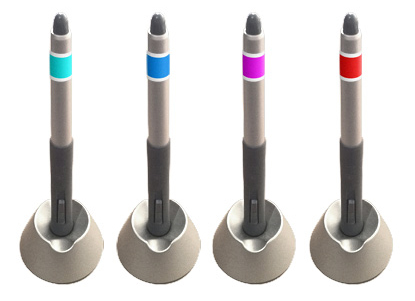
\includegraphics[width=1\linewidth]{gfx/scribblerColors}}
		\caption[Tabletstiftfarben]{Jeder Stift ist eindeutig vom System identifizierbar und hat eine eigene Farbe zugeordnet. Zur Verdeutlichung, wurde jedem Stift ein entsprechend gefärbter Sticker aufgeklebt.}\label{fig:scribblerColors}
\end{figure}

Jeder Stift hat einen Kippschalter an der Seite. Dieser erfüllt in \scribbler die Funktionen >>Undo<< und >>Redo<<, die die letzte Aktion rückgängig machen oder wiederherstellen. 
%sDie Tests haben gezeigt, dass diese Buttons häufig unabsichtlich gedrückt wurden und daher in einer optimalen Version von \scribbler gar nicht mit Funktionen belegt werden sollten.
Stifte werden vom System erst dann wahrgenommen, wenn die Stiftspitze ein bis eineinhalb Zentimeter über das Tablet gehalten werden, wie \autoref{fig:scribblerProximity} demonstriert. Dies ist auf die Hardware zurückzuführen und es kann kein Einfluss darauf genommen werden. Ebenso wird das Drücken des Kippschalters am Stift nur dann registriert, wenn der Stift sich in der entsprechenden Entfernung zum Tablet befindet. Am hinteren Ende eines Stiftes befindet sich ein weiterer Button, der üblicherweise eine Radierfunktion bietet, ähnlich einem mit Radiergummi versehenen Bleistift. Auch \scribbler belegt diese Taste mit einer Radierfunktion, jedoch können damit nur komplette Linien gelöscht werden.

\begin{figure}
        {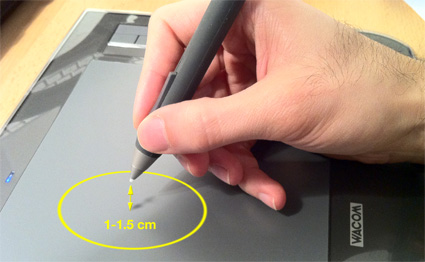
\includegraphics[width=1\linewidth]{gfx/scribblerProximity}}
		\caption[Proximity Event]{Die Hardware erkennt Stifte erst dann, wenn die Spitze ein bis eineinhalb Zentimeter über das Tablet gehalten wird. Das Betriebssystem empfängt dann ein >>Proximity Event<<, das von \scribbler weiterverarbeitet wird.}\label{fig:scribblerProximity}
\end{figure}

\subsection{Grafisches User Interface} \index{Scribbler!GUI}
\scribbler ist ein Dienst, der im Hintergrund läuft und lediglich das Betriebssystem an Funktionalität anreichert. Daher hat es ein sehr subtiles \ac{GUI}, das nahezu vollständig transparent bleibt und Benutzer nicht von ihrer eigentlichen Arbeit ablenkt. Es besteht nur aus einem sternförmigen Icon in der Systemleiste des Betriebssystems, siehe \picref{fig:scribblerIcon}. Dahinter verbirgt sich ein Menü, dargestellt in \picref{fig:scribblerMenu}, das die Funktionen von \scribbler zur Verfügung stellt. Diese können fast alle auch über die Tasten am Tablett durchgeführt werden. Eine Ausnahme bilden der erste Menüeintrag, der \scribbler temporär in einen Standby-Zustand und somit inaktiv setzt, und der letzte Menüeintrag, der das Programm vollständig beendet.

\medskip Benutzer sollen das Programm gar nicht bemerken, müssen aber dennoch ein gewisses Maß an Feedback erhalten, um sinnvoll mit \scribbler arbeiten zu können. Dass der Zeichenmodus aktiv ist, wird Benutzern beispielsweise dadurch mitgeteilt, dass statt dem normalen Pfeil-Cursor (vgl. \picref{fig:scribblerMousePosition}) ein Fadenkreuz-Cursor (vgl. \autoref{fig:scribblerSketching}) angezeigt wird. Zusätzlich markiert \scribbler das aktive Fenster (einer Drittapplikation) mit einem blauen Rahmen. Den Benutzern wird so kommuniziert, welchem Fenster ihre Zeichnungen zugeordnet werden. Man kann sich also vergewissern, ob tatsächlich auf das gewünschte Fenster gezeichnet wird.

\medskip \emph{Scribblers} herausragendstes Feature, das es von allen bisherigen ähnlichen Systemen abhebt, ist der >>Sticky Mode<<. Diese Funktion bewirkt, dass Zeichnungen immer dort bleiben, wo sie hingehören. Wenn ein Benutzer auf ein Fenster zeichnet und dieses nachträglich verschiebt, erkennt \scribbler die Änderung der Fensterposition und verschiebt die Zeichnungen ebenfalls, sodass sie wieder genau dort über dem Fenster liegen, wo sie ursprünglich gezeichnet wurden.

Neben der Fensterposition kann \scribbler auch erkennen, wenn der Benutzer in einem Fenster die Scrollposition ändert. Zeichnet der Benutzer beispielsweise auf ein Element einer Webseite und scrollt dann nach unten oder oben auf der Seite, verschiebt \scribbler wiederum automatisch die Zeichnungen, sodass sie immer an der selben Stelle, relativ zum Inhalt bleiben.

Benutzer erhalten so direktes Feedback vom GUI, da die Zeichnungen in Echtzeit neu positioniert werden und dadurch scheinbar am Fenster haften. Außerdem färbt sich das Programm-Icon in der Systemleiste schwarz (siehe \picref{fig:scribblerMagic}), sobald diese innovativen (nahezu magischen) Funktionen zum Einsatz kommen; ein kleines Detail im Sinne einer besseren User Experience. 

\begin{figure}
	\begin{center}
        \myfloatalign
        \subfloat[Scribbler Icon]
		{\label{fig:scribblerIcon}
        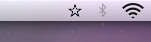
\includegraphics[width=0.47\linewidth]{gfx/scribblerIcon}} \quad
        \subfloat[When magic happens]
        {\label{fig:scribblerMagic}
        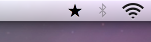
\includegraphics[width=0.47\linewidth]{gfx/scribblerMagic}} \quad
		\subfloat[Scribbler Menu]
		{\label{fig:scribblerMenu}
		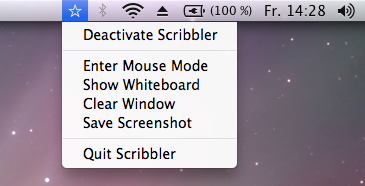
\includegraphics[width=1\linewidth]{gfx/scribblerMenu}} \\
        \caption[Scribbler Menu Icon]{Scribbler Menu Icon}\label{fig:scribblerMenuIcon}
	\end{center}
\end{figure}

\begin{figure}
        {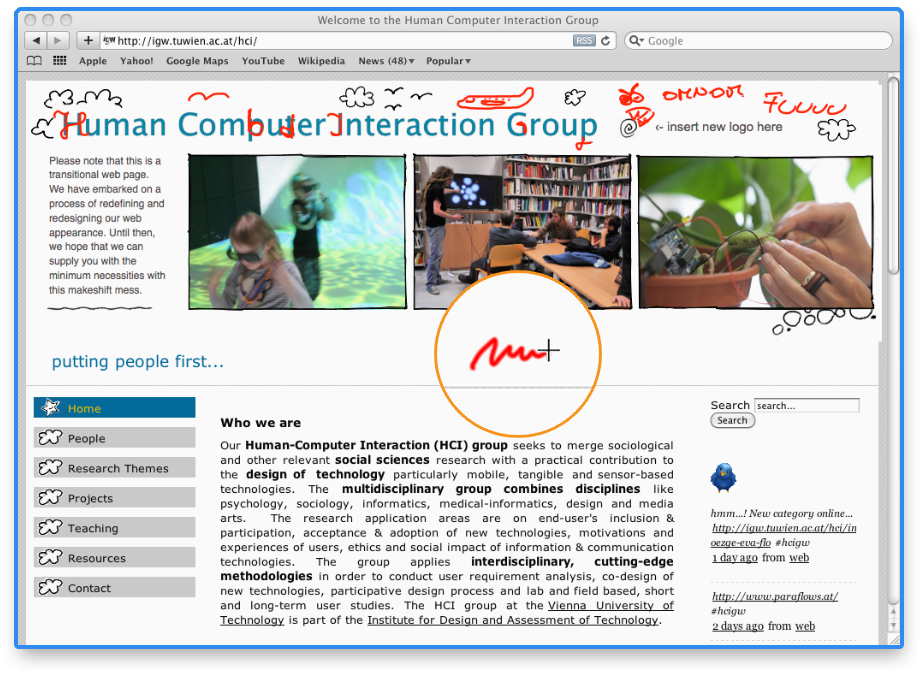
\includegraphics[width=1\linewidth]{gfx/scribblerSketching}}
		\caption[Skizzieren in Scribbler]{Skizzieren in Scribbler}\label{fig:scribblerSketching}
\end{figure}

\subsection{Programmlogik} \label{sec:programmLogik} \index{Scribbler!Programmlogik}
\scribbler wurde auf das von Apple entwickelte \emph{Cocoa}-Framework aufgebaut und genießt somit alle Vorteile einer objektorientierten Programmiersprache. Zusätzlich bietet \emph{Mac OS X} eine Schnittstelle für Bedienungshilfen, sog. Accessibility Daten, die einen wichtigen Teil des Systems ausmachen. Im folgenden Kapitel wird näher auf die Grundfunktionalität von \scribbler eingegangen.

\subsubsection* {Warum weiß Scribbler, wann ein Benutzer zeichnen will?}
\scribbler fängt sogenannte globale und lokale Eingabe-\emph{Events} ab. \emph{Events} sind vom Benutzer ausgelöste Ereignisse, die durch Interaktion mit Eingabegeräten hervorgerufen werden. So ist ein Druck auf die linke Maustaste beispielsweise ein \emph{LeftMouseDownEvent}, oder das Halten einer Taste auf der Tastatur ein \emph{KeyDownEvent}. Geschehen die Aktionen im eigenen Programm, spricht man von lokalen Events. Ereignen sich die Aktionen in anderen Programmen, spricht man von globalen Events. Auf die selbe Weise erkennt das System auch \emph{TabletProximityEvents}. Wie bereits im Punkt \pointref{ssec:hardware} erwähnt, entsteht ein \emph{TabletProximityEvent} wenn ein Stift in die Nähe - mit 1-1.5 cm Abstand - zu einem Tablet kommt (vgl. \autoref{fig:scribblerProximity}). \scribbler wechselt somit automatisch in den Zeichenmodus. 

\bigskip \emph{Anmerkung: \graffito{\(\clubsuit\)} Voraussetzung dafür ist, dass zuvor nicht explizit in den Mausmodus gewechselt wurde.}
\bigskip

\autoref{lst:events} zeigt die Aufrufe, die benötigt werden um globale und lokale Events zu empfangen.

\lstset{language=[Objective]C}
\begin{lstlisting}[float,caption=Global and Local Event Monitoring,label=lst:events]
[NSEvent addGlobalMonitorForEventsMatchingMask: (NSLeftMouseDraggedMask | NSKeyDownMask | NSKeyUpMask | NSTabletProximityMask | NSMouseEnteredMask | NSLeftMouseDownMask | NSOtherMouseDownMask | NSRightMouseDown | NSOtherMouseDownMask)
    handler:^(NSEvent *incomingEvent) {
	
    ...
}];	

[NSEvent addLocalMonitorForEventsMatchingMask: (NSOtherMouseDownMask | NSRightMouseDownMask | NSKeyDownMask | NSKeyUpMask | NSTabletProximityMask)
    handler:^(NSEvent *incomingEvent) {

    ...
}];	
\end{lstlisting}

\subsubsection* {Wie erkennt Scribbler das aktive Programmfenster?} 
Das >>aktive<< Fenster wird in \emph{Mac OS X} auch \emph{Key Window} genannt und bezeichnet das am weitesten vorne liegende Fenster, das gerade den Fokus hat. Leider bietet \emph{Cocoa} oder auch andere Frameworks keine direkte Abfrage nach dem \emph{Key Window}. Es gibt zwar eine sogenannte \emph{WindowList}, in der Informationen über alle offenen Programmfenster abgelegt sind, jedoch ohne Kennzeichnung des aktiven Fensters. \scribbler hat daher einen eigenen Mechanismus, um das aktive Fenster zu finden.

Dazu greift es auf die Daten des aktiven Programms zu und sucht in der \emph{WindowList} nach allen dazugehörigen Einträgen. Da die Einträge der \emph{WindowList} stets nach der Reihenfolge ihres Erscheinens sortiert sind, nimmt \scribbler den Eintrag an erster Stelle und hat somit das aktive Fenster gefunden.

\subsubsection* {Woher weiß Scribbler, wann und wohin sich ein Fenster verschoben hat?}
Immer wenn ein Benutzer ein Programmfenster verschiebt, muss er ein Eingabegerät benutzen. Eine Fensterverschiebung wird naturgemäß durch ein Mausevent, ein sogenanntes \emph{LeftMouseDraggedEvent} ausgelöst. Da \scribbler diese Events empfängt, kann im Anschluss eines solchen Events überprüft werden, ob sich das entsprechende \emph{Key Window} verschoben hat. 

Dazu bedient sich \scribbler an den Informationen, die zu jedem Fenster in der \emph{WindowList} gespeichert werden. Somit können allgemeine Informationen, wie z.B. der Programmname oder auch spezifische, wie die Fenstergröße und -position (zusammengefasst in sog. \emph{Bounds}) gewonnen werden. \autoref{lst:keyWindowHandling} zeigt die Funktionen zur Gewinnung des Programmnamens und der Windowbounds.

\begin{lstlisting}[float,caption=Key Window Handling,label=lst:keyWindowHandling]
// get keyWindow App Name
- (NSString*) getKeyWindowsApplicationName: (NSMutableDictionary*)windowInfos {
	
    return [windowInfos objectForKey:(id)kCGWindowOwnerName];
}
// get keyWindow Bounds
- (NSRect) getKeyWindowBounds: (NSMutableDictionary*) windowInfos {
	
    CGRect rect;
    CFDictionaryRef ref = (CFDictionaryRef)[windowInfos objectForKey:(id)kCGWindowBounds];
    CGRectMakeWithDictionaryRepresentation(ref, &rect);

    return *(NSRect *)&rect;
}
\end{lstlisting}

\begin{figure}
	\begin{center}
        \myfloatalign
        \subfloat[Mouse Position]
        {\label{fig:scribblerMousePosition}
		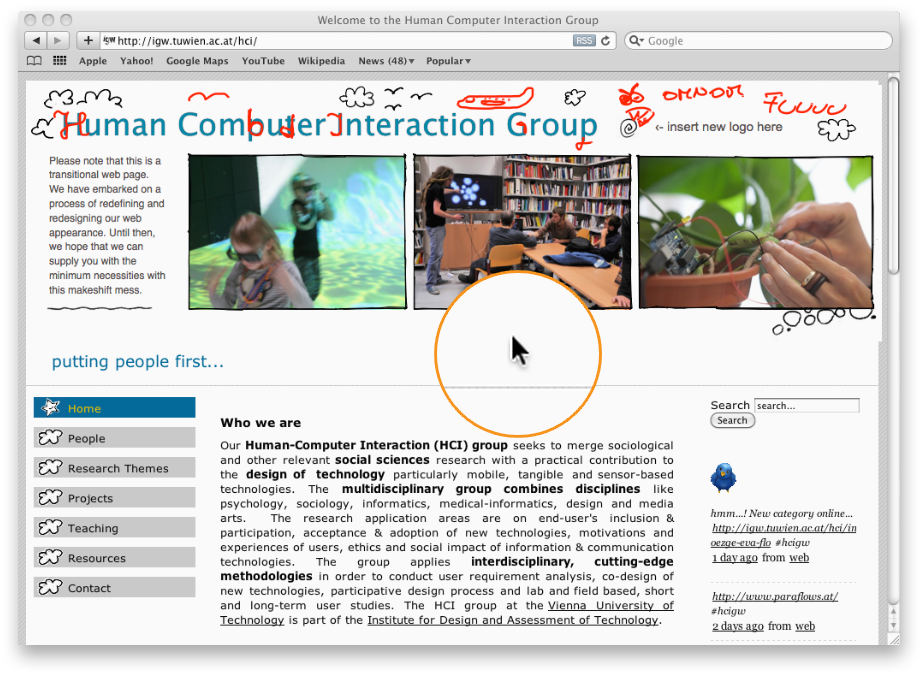
\includegraphics[width=1\linewidth]{gfx/scribblerAccessibility}} \\
        \subfloat[Accessibility Inspector]
        {\label{fig:scribblerAccessibilityInspector}
        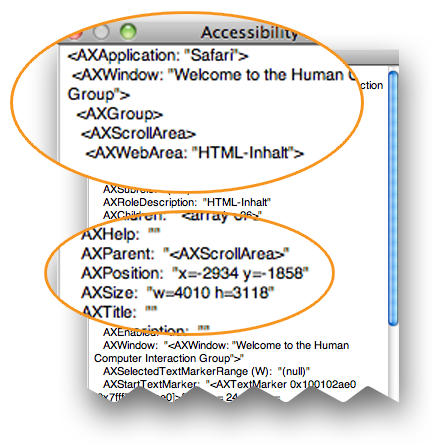
\includegraphics[width=0.7\linewidth]{gfx/scribblerAccessibilityInspector}} \\
        \caption[Accessibility Daten zur aktuellen Mausposition]{Accessibility Daten zur aktuellen Mausposition}\label{fig:scribblerAccessibility}
	\end{center}
\end{figure}

\subsubsection* {Wie können sich die Skizzen beim Scrolling mitbewegen?}
Im Prinzip ist Scrolling dasselbe wie eine Fensterverschiebung: Digitale Inhalte bewegen sich über den Bildschirm. Scrollingaktionen kann man zwar über die bewährten \emph{Events} ansteuern, aber es ist weitaus komplizierter herauszufinden, welche Elemente sich wie weit bewegt haben. Aus Sicherheitsgründen darf ein Programm nicht auf Informationen anderer Programme zugreifen. Wie macht dies dann aber \scribbler?

Hier kommen die anfangs erwähnten Bedienungshilfen bzw. Accessibility Daten ins Spiel. Bedienungshilfen sind Funktionen, die für behinderte Menschen eingeführt worden sind und ausdrücklich in den Systemeinstellungen\footnote{Erreichbar unter Mac OS X: Systemeinstellungen - Bedienungshilfen - >>Zugriff für Hilfsgeräte aktivieren<<.} aktiviert werden müssen. 

\bigskip \emph{Anmerkung: \graffito{\(\clubsuit\)} Scribbler benötigt den >>Zugriff für Hilfsgeräte<< um an Scrollinginformationen anderer Programme zu kommen.}
\bigskip

Unterstützt das aktive Programm Bedienungshilfen, können Accessibility Daten abgerufen werden. Je nach Programmherausgeber unterscheidet sich die Anzahl an verfügbaren Daten. Nicht jedes Programm, das Bedienungshilfen implementiert hat, stellt auch essentielle Daten zur Berechnung von Scrollinginformationen bereit. \autoref{lst:accessiblityDaten} zeigt allgemeine Informationen, die jedoch bei jeder Accessibilitykonfiguration vorhanden sind. So kann durch Bedienungshilfen beispielsweise, auf einfachem Weg das aktive Fenster ermittelt werden. Jedoch nur wenn das aktive Programm Accessibility Daten unterstützt. Welche Accessiblity Daten von einem Programm unterstützt werden, kann mittels dem Dienstprogramm \emph{Accessibility Inspector} herausgefunden werden, das alle verfügbaren Accessibility Daten zu der aktuellen Mausposition anzeigt (siehe \autoref{fig:scribblerAccessibility}). 

\picref{fig:scribblerAccessibilityInspector} zeigt außerdem alle für Scrolling relevanten Einträge. Besitzt \emph{AXParent} das Attribut \emph{AXScrollArea}, existiert ein scrollbarer Bereich innerhalb des aktiven Fensters. Aus den \emph{AXPosition} und \emph{AXSize} Einträgen kann man mittels einfacher Mathematik die aktuelle Scrollingposition errechnen und somit die Bewegung innerhalb des Fensters.

\begin{lstlisting}[float,caption=Laden von Accessibility Daten,label=lst:accessiblityDaten]
_systemWideElement = AXUIElementCreateSystemWide();
	
//Get the app that has the focus
AXUIElementCopyAttributeValue(_systemWideElement, (CFStringRef)kAXFocusedApplicationAttribute, (CFTypeRef*)&_focusedApp);

//Get the window that has the focus
if(AXUIElementCopyAttributeValue((AXUIElementRef)_focusedApp, (CFStringRef)NSAccessibilityFocusedWindowAttribute, (CFTypeRef*)&_focusedWindow) == kAXErrorSuccess) {
    ...
}		
\end{lstlisting}

\section{User Review} \label{sec:userReview} \index{Scribbler!User Review}
Der Prototyp von \scribbler wurde mit verschiedenen potenziellen Nutzern getestet. Darunter drei Designer aus den Bereichen Produkt-, Interaction-, und User Experience Design, die sich an \scribbler in einem reduzierten Setting, also mit nur einem Tablet versuchten. Zusätzlich setzte eine Arbeitsgruppe am Institut für Gestaltungs- und Wirkungsforschung der technischen Universität Wien \scribbler in einem kollaborativen Setting bei einem Projekt-Meeting ein. 

Bei allen drei Sitzungen wurden die Aktionen der Testpersonen durch eine Videokamera gefilmt und ihre Kommentare auf einem Tonträger festgehalten. Die drei Designer wurden zusätzlich interviewt, und die Transkripte sind im Appendix im Kapitel \nameref{ch:interviews} zu finden.

Es folgt nun positives und kritisches Feedback, das aus diesen Tests hervorgegangen ist.

\subsection{Positives Feedback}

\scribbler wurde von den Testpersonen durchwegs positiv aufgenommen und alle waren interessiert an Konzept und Funktionsweise. Die Arbeitsgruppe am Institut für Gestaltungs- und Wirkungsforschung der Technischen Universität Wien konnte den Prototypen produktiv bei ihrem Projekt-Meeting einsetzen und die Idee hinter \scribbler wurde als sinnvoll erachtet. 

Peter, Produktdesigner und Dozent an der Universität für Angewandte Kunst Wien, bewertete das Konzept von \scribbler sehr gut.

\begin{extract}[Peter, Produktdesigner, über \scribbler.]
	{
		\myfloatalign
		\begin{tabularx}{\textwidth}{p{1.5cm}X}
    		Peter  & Für mich ist das auf jeden Fall eine Traumsituation, da ich jetzt schon Notizen zu Präsentationen mache. Nur das Problem ist eben jetzt, dass ich die Notizen auf Zetteln mache und mir dazuschreiben muss, zu welcher Zeichnung die Notizen gehören, damit ich sie nachträglich wieder zuordnen kann.
		\end{tabularx}
	}
	\captionX{Traumsituation}
\end{extract}

Peter könnte sich vorstellen, das Tool im Unterricht im kollaborativen Setting einzusetzen und erklärt, in welchen spezifischen Situationen \scribbler nützlich wäre und in welchen nicht.

\begin{extract}[Peter über den Einsatz von \scribbler im Unterricht.]
	{
		\myfloatalign
		\begin{tabularx}{\textwidth}{p{1.5cm}X}
    		Peter & Ja das wäre super, wenn ich das im Unterricht einsetzen könnte. Es wäre spitze wenn jeder die Möglichkeit hätte, mitzuarbeiten. Wobei ich nicht ganz sicher bin ob Darstellungstechnik das passende Unterrichtsfach für \scribbler ist, weil da geht es konkret um das Zeichnen und dann reichen Grobskizzen leider nicht aus, sondern man muss schon detaillierte Zeichnungen anfertigen. Anders sieht es da bei Designvisualisierungen aus, die auch in meinem Unterricht vorkommen. Da wäre es wirklich cool, die Studenten direkt einzubinden. Jeder könnte auch Stichworte dazuschreiben und ähnlich einem Brainstorming vernetzen. Das könnte ich mir gut vorstellen. 
		\end{tabularx}
	}
	\captionX{Einsatz im Unterricht}
\end{extract}

Jedem Stift eine eigene Farbe zuzuweisen gefällt Peter gut. Für seine Zwecke benötigt er mehr als nur eine Farbe und dies erscheint ihm eine gute Lösung. Er weist jedoch auch darauf hin, dass er gerne Kontextmenüs in Zeichenprogrammen verwendet und so schneller zwischen verschiedenen Farben wechseln kann.

\begin{extract}[Jedem Stift wird eine eigene Farbe zugewiesen.]
	{
		\myfloatalign
		\begin{tabularx}{\textwidth}{p{1.5cm}X}
    		Clemens & Du zeichnest derzeit mit der Farbe Magenta. Du hast vorher gemeint für Grobskizzen reicht dir eine Farbe oder?\\

			Peter & Also wenn ich in der Strukturierungsphase bin, wäre es schon gut wenn ich mehrere Farben hätte.\\

			Clemens & Ok. Dazu haben wir eigentlich mehrere Stifte mit unterschiedlichen Farben angedacht.\\

			Peter & Wirklich wahr?\\

			 & \emph{(Peter greift zu einem anderen Stift und probiert ihn aus)}\\

			Peter & Wahnsinn. Ja, das finde ich super wenn man das so löst.\\

			Thomas & Wir haben uns gedacht wir halten uns daran, möglichst realitätsnahe zu bleiben. Beim Zeichnen auf Papier würdest du auch einen anderen Stift zur Hand nehmen.\\

			Peter & Verstehe. Was ich irrsinnig gerne verwende sind Untermenüs bzw. Popupmenüs. Das gibt es bei verschiedenen Programmen. Wenn ich z.B. auf die Stifttaste drücke geht ein Untermenü auf. So wie bei >>Autodesk Maya<< oder >>Sketchbook<<. Das sind Programme in denen ich z.B. immer zeichne. Und da hätte man im Untermenü auch die Möglichkeit auf eine Farbpalette, oder vielleicht auch 2-3 verschiedene Strichstärken. Dazu drück ich auf die Stifttaste, fahre mit dem Stift auf das Menü, lass wieder aus, das Menü ist wieder weg und ich habe die neue Einstellung. Beim Zeichnen ist das super; das ist etwas was mir z.B. in Photoshop abgeht.
		\end{tabularx}
	}
	\captionX{Farben}
\end{extract}

Das Whiteboard, das in \scribbler eingeblendet werden kann und dazu dient, auf eine weiße Fläche statt einem bestimmten Fenster zu zeichnen, wurde von allen Testpersonen positiv bewertet. Es gibt Situationen, in denen man schnell etwas aufkritzeln möchte, das nicht mit dem Fensterkontext in Verbindung steht, beispielsweise eine spontane Idee für ein Konzept oder ein Design. In diesen Momenten bietet \scribbler die passende Funktion, und die Idee kann so abseits vom aktuellen Geschehen festgehalten und später wieder abgerufen werden.

Durch \scribbler ist es möglich, auf mehrere nebeneinander angeordnete Fenster des Desktops zu zeichnen und dadurch semantische Verbindungen herzustellen. Dadurch können Inhalte auf eine ganz neue Art und Weise präsentiert werden. Derzeit ist es so, dass Zeichnungen sich immer an das aktive Fenster, beispielsweise das Browserfenster heften und ihre Position relativ zur Fenster- und Scrollposition mitbewegen.

\begin{extract}[Zeichnungen heften sich an das aktive Fenster, auch wenn außerhalb dessen gezeichnet wird.]
	{
		\myfloatalign
		\begin{tabularx}{\textwidth}{p{1.5cm}X}
    		Thomas & Habe ich es richtig verstanden, dass du es gerne so hättest, dass wenn mehrere gleichzeitig zeichnen, jeder auf sein eigenes Fenster zeichnet und die jeweiligen Zeichnungen auf dem eigenen Fenster kleben bleiben? Momentan hängen alle Zeichnungen - egal von wem gezeichnet - nur auf dem aktivem Fenster. Sobald du das Fenster verschiebst, verschiebst du die Zeichnungen mit.\\

			 & \emph{(Peter denkt nach)}\\

			Peter & Weiß ich nicht. Also für mich funktioniert das derzeit von der Überlegung her recht gut. Aber ich müsste es erst länger ausprobieren, um auch die wirklichen Stärken zu finden.
		\end{tabularx}
	}
	\captionX{Zugehörigkeit}
\end{extract}

Als Produktdesigner zeichnet Peter sehr viel und er tut dies auch während Besprechungen. Das Zeichnen hilft ihm mit den anderen zu kommunizieren und bringt seine Kreativität in Schwung. 

\begin{extract}[Zeichnen um besser zu kommunizieren.]
	{
		\myfloatalign
		\begin{tabularx}{\textwidth}{p{1.5cm}X}
			Peter & Was hier (in \scribbler) auch gut funktioniert, ist das Verdeutlichen von Ideen. Ich bin jemand, der irrsinnig gerne zeichnet zum Reden. Ich könnte so z.B. ein paar Punkte rausholen und einen Teil, der hier im Bereich unten schwer zu erkennen ist, noch einmal rauszeichnen.
		\end{tabularx}
	}
	\captionX{Kommunikation}
\end{extract}

Deshalb sieht er für \scribbler gute Einsatzmöglichkeiten bei Brainstormings und in Ideenfindungsphasen. Dadurch können Konzepte und Ideen schnell und effizient vermittelt und Inspiration gefördert werden. Ebenfalls denkbar wäre für ihn der Einsatz von \scribbler in Graphic-Recording-Meetings. Es handelt sich dabei um Sitzungen, bei denen eine Person jegliche verbale Kommunikation in der Gruppe als Skizzen festhält.

\begin{extract}[Ein Einsatz bei Graphic-Recordings wäre denkbar.]
	{
		\myfloatalign
		\begin{tabularx}{\textwidth}{p{1.5cm}X}
			Peter & Das ist eine recht interessante Geschichte. Es handelt sich um Leute, die Meetings mit zeichnen. Das passiert analog auf einem Blatt Papier mit Stift. Nehmen wir an da sitzen mehrere Techniker und andere in ein Projekt verwickelte Personen, die Konzepte verbal besprechen und dann gibt es einen Zeichner, der, während die Leute ihre Ideen artikulieren, diese direkt zu Papier bringt und aufzeichnet. Darauf baut dann die Diskussion weiter auf und die Teilnehmer können gleich auf die Skizzen eingehen und sie weiter entwickeln oder verwerfen. Am Ende kann man anhand der Bilder nachvollziehen, worüber gesprochen worden ist. Das wäre sicherlich auch ein Gebiet, bei dem man \scribbler oder ähnliche Anwendungen zum Einsatz bringen könnte.
		\end{tabularx}
	}
	\captionX{Graphic-Recording}
\end{extract}

\scribbler könnte diese Art von Meetings unterstützen, indem die Skizzen und Zeichnungen, die die verbale Kommunikation der Sitzung abbilden, auf digitalem Wege erstellt werden. Dadurch wäre es leichter, Kopien anzufertigen und für jeden Teilnehmer bereitzustellen. Außerdem könnten sie in digitaler Form auch gleich per E-Mail versendet werden. \scribbler könnte außerdem das Meeting sinnvoll ergänzen. Beispielsweise, die Teilnehmer besprechen verschiedene Webseiten oder Produkte der Konkurrenz, so könnte der Zeichner diese Seiten öffnen und direkt darauf die Skizzen des Meetings festhalten. Auf diese Weise würde sich ein konkreter Kontext manifestieren. Folglich könnten mehr Informationen gesammelt werden.

\subsection{Kritisches Feedback}
Die Testdurchläufe mit den potentiellen Benutzern haben nicht nur positive, sondern auch kritische Aspekte von \scribbler enthüllt. Einige davon waren uns bereits vor dem Testen bewusst und wurden durch die Tests und Interviews bestätigt. Andere Kritikpunkte waren komplett neue Einsichten und haben uns auf wichtige Dinge aufmerksam gemacht. Die verschiedenen kritischen Anmerkungen werden im folgenden verschiedenen Kategorien zugeordnet, um ein besseres Verständnis zu bieten.

\subsubsection{Unvollständigkeit des Prototypen}
Als \scribbler von der Arbeitsgruppe am Institut für Gestaltungs- und Wirkungsforschung in einem kollaborativen Setting eingesetzt wurde, wollten alle Teilnehmer sofort die Zeichenfunktion ausprobieren. Gleichzeitig griffen alle zum Stift und bemerkten dann, dass der Prototyp jeweils nur einem und nicht mehreren Benutzern zu zeichnen erlaubt. Schon zu Beginn des Projektes wurde deutlich, dass dies eines der wichtigsten Features von \scribbler sein würde, aber es war nicht möglich, dieses in der kurzen Entwicklungszeit zu implementieren. Dieses Feature erfordert die Implementierung multipler Cursor und ist technisch aufwändig. Fehlt es jedoch, kommt es zu einem >>Flaschenhalseffekt<<, der die Effizienz von Meetings stark einschränkt. Personen können nicht parallel zeichnen, bzw. arbeiten und sind so ständig gezwungen, die Aktionen der anderen abzuwarten. Hinzu kommt ein erhöhter Aufwand der Absprache untereinander zur Koordination der Tätigkeiten. Der Test hat gezeigt, dass die Teilnehmer des Meetings sich ständig absprechen müssen, wer wann zeichnen kann. Diese zusätzliche Koordination ist in herkömmlichen Meetings überhaupt nicht notwendig und stellt einen klaren Nachteil hinsichtlich der Effizienz der Sitzung dar. Die Befürchtung, die bereits vor dem Test aufgekommen war, wurde sehr schnell bestätigt. Bei einer Weiterentwicklung von \scribbler muss diesem kritischen Feature höchste Priorität zugeordnet werden, denn es entscheidet über Erfolg oder Misserfolg des gesamten Systems.

\medskip Häufig kam es vor, dass Testpersonen unabsichtlich den Kippschalter am Stift drückten. Dies führte dazu, dass die letzte Aktion rückgängig gemacht wurde. Dieses Problem war uns schon während der Implementierungsphase bei internen Tests aufgefallen. Personen, die selten oder nie Tablet und Stift als Eingabegerät verwenden, passiert dieses unabsichtliche Drücken der Undo-Taste immer wieder. Der Produktdesigner, der täglich mit dem Tablet arbeitet, hatte hingegen keine Schwierigkeiten. Um \scribbler für eine breite Masse benutzbar zu machen, muss bei einer Weiterentwicklung darauf geachtet werden, dass den Tasten des Stifts keine Funktionen zugewiesen werden. Stattdessen sollten diese sinnvoll auf den Tasten des Tablets selbst angeordnet werden.

\medskip Es wurde sehr schnell deutlich, dass die Einsatzmöglichkeiten von \scribbler begrenzt sind. Die wenigen Zeichenfunktionen reichen lediglich für grobe Skizzen und Kritzeleien aus. \scribbler muss hier gezielt an Funktionalität angereichert werden und zumindest optional Features wie Strichstärke oder Druckempfindlichkeit anbieten.

\begin{extract}[Die Einsatzmöglichkeiten sind begrenzt.]
	{
		\myfloatalign
		\begin{tabularx}{\textwidth}{p{1.5cm}X}
			Thomas & Sind diese primitiven Zeichenmöglichkeiten ausreichend, oder fehlt dir da was?\\
			Peter & Nein, für Darstellungstechnik reichen diese Möglichkeiten bei weitem nicht aus. Man braucht da Dinge wie Strichstärke, gerade Linien, etc. Das sind Sachen, die Photoshop kann und die sind auch wirklich notwendig. Aber bei solchen groben Sachen, wie ich sie hier jetzt am Screen gezeichnet habe kann das schon reichen. Wichtig ist natürlich auch die Transparenz von Linien. Beim Skizzieren beginnt man ja mit ganz leichten Strichen, die das grobe Grundgerüst darstellen und zeichnet dann mit mehr Druckstärke drüber, sodass die Linien deutlicher werden und die Skizze konkreter wird.
		\end{tabularx}
	}
	\captionX{Fehlende Funktionalität}
\end{extract}

Der Prototyp war noch fehleranfällig und stürzte gelegentlich ab oder zeigte unerwartetes Verhalten. Dies wurde von den Teilnehmern zwar kritisiert, alle zeigten jedoch Verständnis für die unfertige Teilimplementierung. Selbstverständlich muss die finale Version von \scribbler stabil laufen und darf keine Daten verlieren.


\subsubsection{Technische Probleme}
Eine große technische Hürde stellt für \scribbler das Speichern von Daten zur späteren Wiederverwendung dar. \scribbler hat natürlich keinen Einfluss auf andere Programme, hängt aber vollständig von deren Kontext ab. Das bedeutet, dass Zeichnungen in \scribbler nur dann sinnvoll sind, wenn die Fenster von Drittprogrammen darunter liegen. Die Problematik der Abspeicherung wird hier sehr schnell deutlich: \scribbler kann die Fenster und Anordnung von Drittprogrammen nicht speichern. Im Prototypen gibt es eine Funktion, die ein Bild des Desktops mit allen daraufliegenden Zeichnungen erstellt und in einer Datei am Schreibtisch ablegt. Dieses Rasterbild kann jedoch nicht weiterverwendet werden. Außerdem müssen bei längerem Arbeiten mit \scribbler sehr viele Bilder angefertigt werden, um alle Zeichnungen abzubilden. Dabei füllt sich der Desktop sehr schnell und zu einem späteren Zeitpunkt müssen Benutzer sich mit unzähligen Dateien plagen. Es muss hier dringend ein passendes Konzept gefunden werden, das die Bedürfnisse besser deckt als einfache Rasterbilder. 

\medskip Das Schreiben ist eine weitere Schwäche von \scribbler. Die prototypische Implementierung ist technisch nicht optimiert und das System zeichnet nur wenige Bewegungspunkte des Stifts am Tablet auf. Dadurch entstehen ungenaue Linien und Handschrift wird deutlich unlesbar. Gerade wenn Benutzer versuchen, auf kleine Flächen zu schreiben, scheitern sie in den meisten Fällen. \scribbler und der darunter liegende Code muss soweit optimiert werden, dass es möglich wird, auf Fenster in annehmbarer Größe zu schreiben, weil dies ein sehr übliches Szenario darstellt.

\medskip Die Entscheidung, Tablets ohne integriertes Display als Hardware für \scribbler zu benutzen, fiel aus der Annahme heraus, dass Personen in kollaborativen Settings weniger miteinander interagieren würden, wenn jeder auf seinen eigenen Bildschirm schaut. Ziel war der Einsatz eines einzelnen großen Displays, um eine größere Gemeinsamkeit zu schaffen und Teamwork zu fördern. Vielen Benutzern fällt jedoch die Abstraktion von Tablet hin zu einem entfernten Display schwer. Sie schaffen es nur sehr schwer, ihre Bewegungen mit dem Stift am Tablet so zu koordinieren, dass am Display auch tatsächlich die beabsichtigten Striche gezeichnet werden. Bereits das Einkreisen von gewissen Elementen am Bildschirm kann schwierig erscheinen und Frust beim Benutzer erzeugen. Diese Problematik verschärft sich, wenn das Display sich nicht frontal, sondern seitlich zum Benutzer befindet. Sitzt dieser zusätzlich vor dem Tablet, wird es fast unmöglich, \scribbler sinnvoll zu nutzen.

\subsubsection{Konzeptionelle Probleme}
\scribbler setzt den Einsatz von spezieller Hardware voraus. Benötigt wird ein großes Display oder ein Beamer, ein starker Rechner mit dem Betriebssystem OS X und mehrere Wacom Tablets. Diese Komponenten sind zum einen teuer und zum anderen keine üblichen Geräte, die die meisten Betriebe im Inventar führen. Aus diesen Gründen ist der Einsatz von \scribbler nicht ohne weiteres möglich, beispielsweise vor Ort beim Kunden. Dieser Aufwand steht in keinem Verhältnis zum effektiven Nutzen innerhalb eines Meetings steht.

\begin{extract}[Notwendige Hardware schränkt ein.]
	{
		\myfloatalign
		\begin{tabularx}{\textwidth}{p{1.5cm}X}
			Zed & \emph{[...]} Beim kollaborativen Zusammenarbeiten mit dem Kunden glaub ich nicht dass es funktionieren würde. Der Kunde kann das nicht bedienen, allein der Umgang mit dem Tablet ist eher komplex. Hinzu kommt die notwendige Hardware, die ja auch erst ein mal angeschafft werden muss und transportiert werden muss. Man benötigt dann ja mehrere Tablets. 
		\end{tabularx}
	}
	\captionX{Transport und Kosten}
\end{extract}

Für die Interaction- und User Experience Designer scheint \scribbler keine wirklich brauchbaren Szenarios und Einsatzmöglichkeiten zu bieten.

\begin{extract}[Der praktische Nutzen erschließt sich nicht jedem.]
	{
		\myfloatalign
		\begin{tabularx}{\textwidth}{p{1.5cm}X}
			Zed & Aber ich kann mir auch den praktischen Nutzen nicht so recht vorstellen. Zu sagen, ich würde das System wirklich irgendwo einsetzen... ich weiß nicht. Das Szenario fehlt mir. Beim Kunden fällt das nämlich komplett flach.
		\end{tabularx}
	}
	\captionX{Nutzen}
\end{extract}

Gewisse zusätzliche Features und Optimierungen würden das \scribbler Konzept jedoch interessanter für sie erscheinen lassen.

\begin{extract}[Notwendige Funktionalität.]
	{
		\myfloatalign
		\begin{tabularx}{\textwidth}{p{1.5cm}X}
			Thomas & Was wäre notwendig, um es für dich nutzbar zu machen?\\
			Zed & Dieser komischer Hovereffekt des Stifts am Tablet bereitet mir Schwierigkeiten. Das müsste man auf jeden Fall irgendwie lösen. Sodass man das Gefühl bekommt, dass man wirklich exakt arbeiten kann mit dem Ding. Das fehlt mir. Schön wäre natürlich auch, wenn man die Übersetzung von Tablet auf Screen lösen könnte, wobei das natürlich nur dann geht, wenn der Screen im Tablet integriert ist. Auch cool wäre, wenn man über das Internet zusammenarbeiten könnte, denn so ist man an dieses Setting im Raum gebunden, nicht mal über ein lokales Netzwerk hat man da irgendwelche Freiheiten.
		\end{tabularx}
	}
	\captionX{Nutzbar machen}
\end{extract}

Die Entscheidung, Linien in \scribbler als Vektorobjekte zu speichern, ging mit einigen negativen Konsequenzen einher. So ist zum Beispiel die Radiergummifunktion eingeschränkt. \scribbler kann immer nur eine ganze Linie komplett löschen. Folglich muss der Benutzer eine Linie vollständig löschen und neu zeichnen. Angenommen der Benutzer möchte wirklich nur eine Linie kürzen, die etwas zu lang geworden ist, so muss er sie löschen und neu zeichnen. 

\begin{extract}[Der Radierer löscht nur ganze Linien.]
	{
		\myfloatalign
		\begin{tabularx}{\textwidth}{p{1.5cm}X}
			Clemens & \emph{[...]} Die Möglichkeit zu Radieren gibt es eigentlich auch - die hintere Taste am Stift dient dazu. Doch da das Programm vektorbasierend ist, radiert es nur den letzten Strich. Ist diese Funktion zu wenig für deinen Gebrauch?\\
			Peter & Also wenn ich wirklich an einem Produkt arbeite, um eine Form herauszuarbeiten, wäre es zu wenig ja. Aber um einfache Sachen, wie z.B Notizen einzufügen oder Ideen zu formulieren, funktioniert es schon. Man müsste aber vielleicht anfangen das Programm häufiger zu verwenden, um ein gutes Feedback abgeben zu können.
		\end{tabularx}
	}
	\captionX{Radieren}
\end{extract}

\subsubsection{Wünsche der Benutzer}
Offensichtliche Verbesserungen, wie Druckempfindlichkeit, Strichstärke und konkretere Zeichenmöglichkeiten wurden von fast allen Teilnehmern angesprochen. Zusätzlich gab es einige Einwände und Ideen zu Features, die das Nutzungserlebnis von \scribbler verbessern könnten. Essenziell für ein effizientes Arbeiten mit \scribbler erscheint die Möglichkeit, Zeichnungen nachträglich am Bildschirm noch verschieben zu können. So können erst Ideen generiert und danach Ordnung und Struktur geschaffen werden.

\begin{extract}[Es wäre gut, wenn man Zeichnungen verschieben könnte.]
	{
		\myfloatalign
		\begin{tabularx}{\textwidth}{p{1.5cm}X}
			Thomas & Ich habe gesehen, du würdest dir auch wünschen dass du einzelne Teile von Zeichnungen wo anders hinschieben könntest oder? Also dass du einen bestimmten Bereich ausschneiden und verschieben könntest.\\
			Peter & Ja, das wäre vielleicht speziell bei der Ideenfindung, wo alles durcheinander steht, oder auch bei Skizzen in einem Brainstorming technischer Natur interessant. Weil meistens ist der zweite Schritt dann der, dass ich anfange die Ideen zu ordnen. Also es wäre gut, um den ersten Prozess der Ideenfindung nicht zu stoppen bzw. ihm eine Hürde zu geben, sondern gleich weiterarbeiten zu können. Und da ist es eben notwendig das Ganze in eine Ordnung zu bringen. Dann hätte ich wirklich eine Lösung wo alle gemeinsam arbeiten können.
		\end{tabularx}
	}
	\captionX{Verschieben}
\end{extract}

Pi und Zed hatten die Idee, zusätzlich ein Trackpad anstatt einer Maus zusammen mit dem Tablet als Eingabegeräte zu nutzen. Das Tablet wäre nur für Schreiben und Zeichnen zuständig, während das Trackpad zu Positionierung des Cursors genutzt werden könnte. Eventuell würde man so die Steuerung für Benutzer optimieren, die im Umgang mit Tablets ungeübt sind.

\begin{extract}[Ein Trackpad statt einer Maus könnte die Eingabe erleichtern.]
	{
		\myfloatalign
		\begin{tabularx}{\textwidth}{p{1.5cm}X}
			Pi & Vielleicht ist die relative Projektion des Tablets dann sinnvoll, wenn man zwei Eingabegeräte verwendet. Dann setze ich mit der Maus den Zeiger dorthin, wo ich ihn möchte und kann sofort dort los zeichnen, egal wo am Tablet sich mein Stift befindet. \emph{[...]} Oder man könnte auch überhaupt zwei Tablets haben, das eine zur Steuerung mit Gesten und das andere zum Zeichnen.\\
			 & \emph{[...]}\\
			Zed & Da würde sich doch das Magic Pad von Apple anbieten.
		\end{tabularx}
	}
	\captionX{Trackpad}
\end{extract}

Von allen drei Designern wurde der Wunsch nach einer Online-Funktion geäußert. Sie alle haben schon öfter die Erfahrung gemacht, mit anderen Kollegen über das Internet zusammenzuarbeiten und es würde sich anbieten, \scribbler dafür zu nutzen. Für die lokale Benutzung würden sich die beiden auch wünschen, dass nicht nur die Zeichnungen des aktiven Fensters sondern jene von inaktiven Fenstern im Hintergrund angezeigt werden. Um Chaos auf dem Bildschirm zu vermeiden könnte man beispielsweise Zeichnungen im Hintergrund in Grau und mit verschiedenen Alpha-Werten, entsprechend dem Z-Index des zugehörigen Fensters anzeigen.

\begin{extract}[Es sollten nicht nur Zeichnungen des aktiven Fensters dargestellt werden.]
	{
		\myfloatalign
		\begin{tabularx}{\textwidth}{p{1.5cm}X}
			Zed & Das heißt es hängt alles an einem Fenster dran... hmmm, kannst du mal bitte das hintere Fenster aktivieren und es so verschieben, dass man die Fenster und Zeichnungen dahinter sieht?\\
			Thomas & Hmm, das geht so nicht. Es werden immer nur die Zeichnungen auf dem aktiven Fenster angezeigt.\\
			Zed & Ah, hmm. Ich glaub das irritiert mich, dass die Zeichnungen verschwinden. Vielleicht sollte man die ausgegraut anzeigen, so wie die inaktiven Fenster selbst.\\
			Clemens & Es besteht dann die Gefahr, dass ein Chaos entsteht, wenn zu viele Linien angezeigt werden.\\
			Zed & Ja stimmt, aber man könnte doch mit verschiedenen Alpha-Werten arbeiten, je nach dem, wie weit hinten sich ein Fenster befindet.\\
			Thomas & Oh, ja das klingt nach einer guten Idee.\\
			Pi & Man könnte dadurch den Kontext wahren und sehen was man bereits gemacht hat.
		\end{tabularx}
	}
	\captionX{Inaktive Fenster}
\end{extract}

Zudem kam bei ihnen der Wunsch nach einer besseren Darstellung der Zugehörigkeit von Zeichnungen zu Fenstern auf. Eine Idee wäre Farbe dafür einzusetzen, jedoch würde dies wiederum die Freiheit beim Zeichnen einschränken, da keine beliebigen Farben mehr gewählt werden könnten. Auch eine Darstellung, wer welche Zeichnungen gemacht hat, sollte es geben. Im Testsetting, das die Arbeitsgruppe an der Universität eingesetzt hat, wurde dies so gelöst, dass jedem Tablet eine Farbe zugewiesen wurde. Zu jedem gab es mehrere Stifte, die unterschiedliche Helligkeitswerte mit dem Farbwert des Tablets kombinierten. So konnte zumindest etwas Variation eingebracht werden. Im kollaborativen Setting wäre es ebenfalls wünschenswert, wenn mehrere Benutzer gleichzeitig auf verschiedene Fenster zeichnen könnten und die Zeichnungen dem jeweiligen darunter liegenden Fenster zugeordnet werden könnten. Dies stellt natürlich eine große technische Hürde dar und bei einer Weiterentwicklung von \scribbler muss die Machbarkeit erst exploriert werden.

Peter, der Produktdesigner, würde außerdem ein Kontextmenü benötigen, das ihm ein paar Optionen anbietet. Gängige Skizzierprogramme bieten diese Funktion an und ermöglichen so eine sehr hohe Effizienz bei der Arbeit.

\section{Achievements} \index{Scribbler!Achievements}
Abschließend werden kurz die im Abschnitt \pointref{sec:anforderungen} beschriebenen Anforderungen an ein kollaboratives Skizziertool, den umgesetzten Merkmalen von \scribbler gegenübergestellt. Die Merkmale von \scribbler werden wiederum in die vier Einflussfaktoren \emph{Hardware}, \emph{Software}, \emph{Kollaboration} und \emph{Skizzieren} eingeteilt.  \autoref{fig:scribblerAnforderungsauswertung} veranschaulicht diese durch eine farbliche Kennzeichnung der ursprünglichen Erkenntnisse aus der Literatur. In Grün gehaltene Erkenntnisse wurden in der Betaversion von \scribbler bereits behandelt, rot eingefärbte konnten (noch) nicht umgesetzt werden.

\medskip Wie die Abbildung erkennen lässt, konnte ein Großteil der Anforderungen umgesetzt werden, konkret 17 Punkte (77,27\%). Die restlichen 5 Punkte (22,73\%) blieben vorwiegend durch technische Probleme bis dato ungelöst.

\subsubsection*{Hardware} 
Durch das Benutzen von Grafiktablets in Verbindung mit einem Flatscreen, wurde laut Lee ein solides Setting für das System geschaffen und die Weichen für eine Whiteboardfunktion gelegt. Die zwei Hauptmodi von \scribbler, der \emph{Zeichenmodus} und der \emph{Mausmodus}, können explizit durch Tabletbuttons gewechselt werden. Beobachtungen zeigten, dass dies den Arbeitsfluss beschleunigte.

Das derzeit schwerwiegenste Problem von \scribbler ist jedoch die Tatsache, dass das System nur einem Benutzer erlaubt, digitale Inhalte zu bearbeiten und nicht allen gleichzeitig. Die Userreviews zeigten ganz klar den Wunsch nach dieser Funktion. Nur so können Koordinationsschwierigkeiten vermindert werden. 

Ebenso wurde deutlich, dass besonders Benutzer mit wenig Tableterfahrung, Probleme bei der Benutzung der Buttons an den Tabletstiften haben.

\begin{figure}
	        {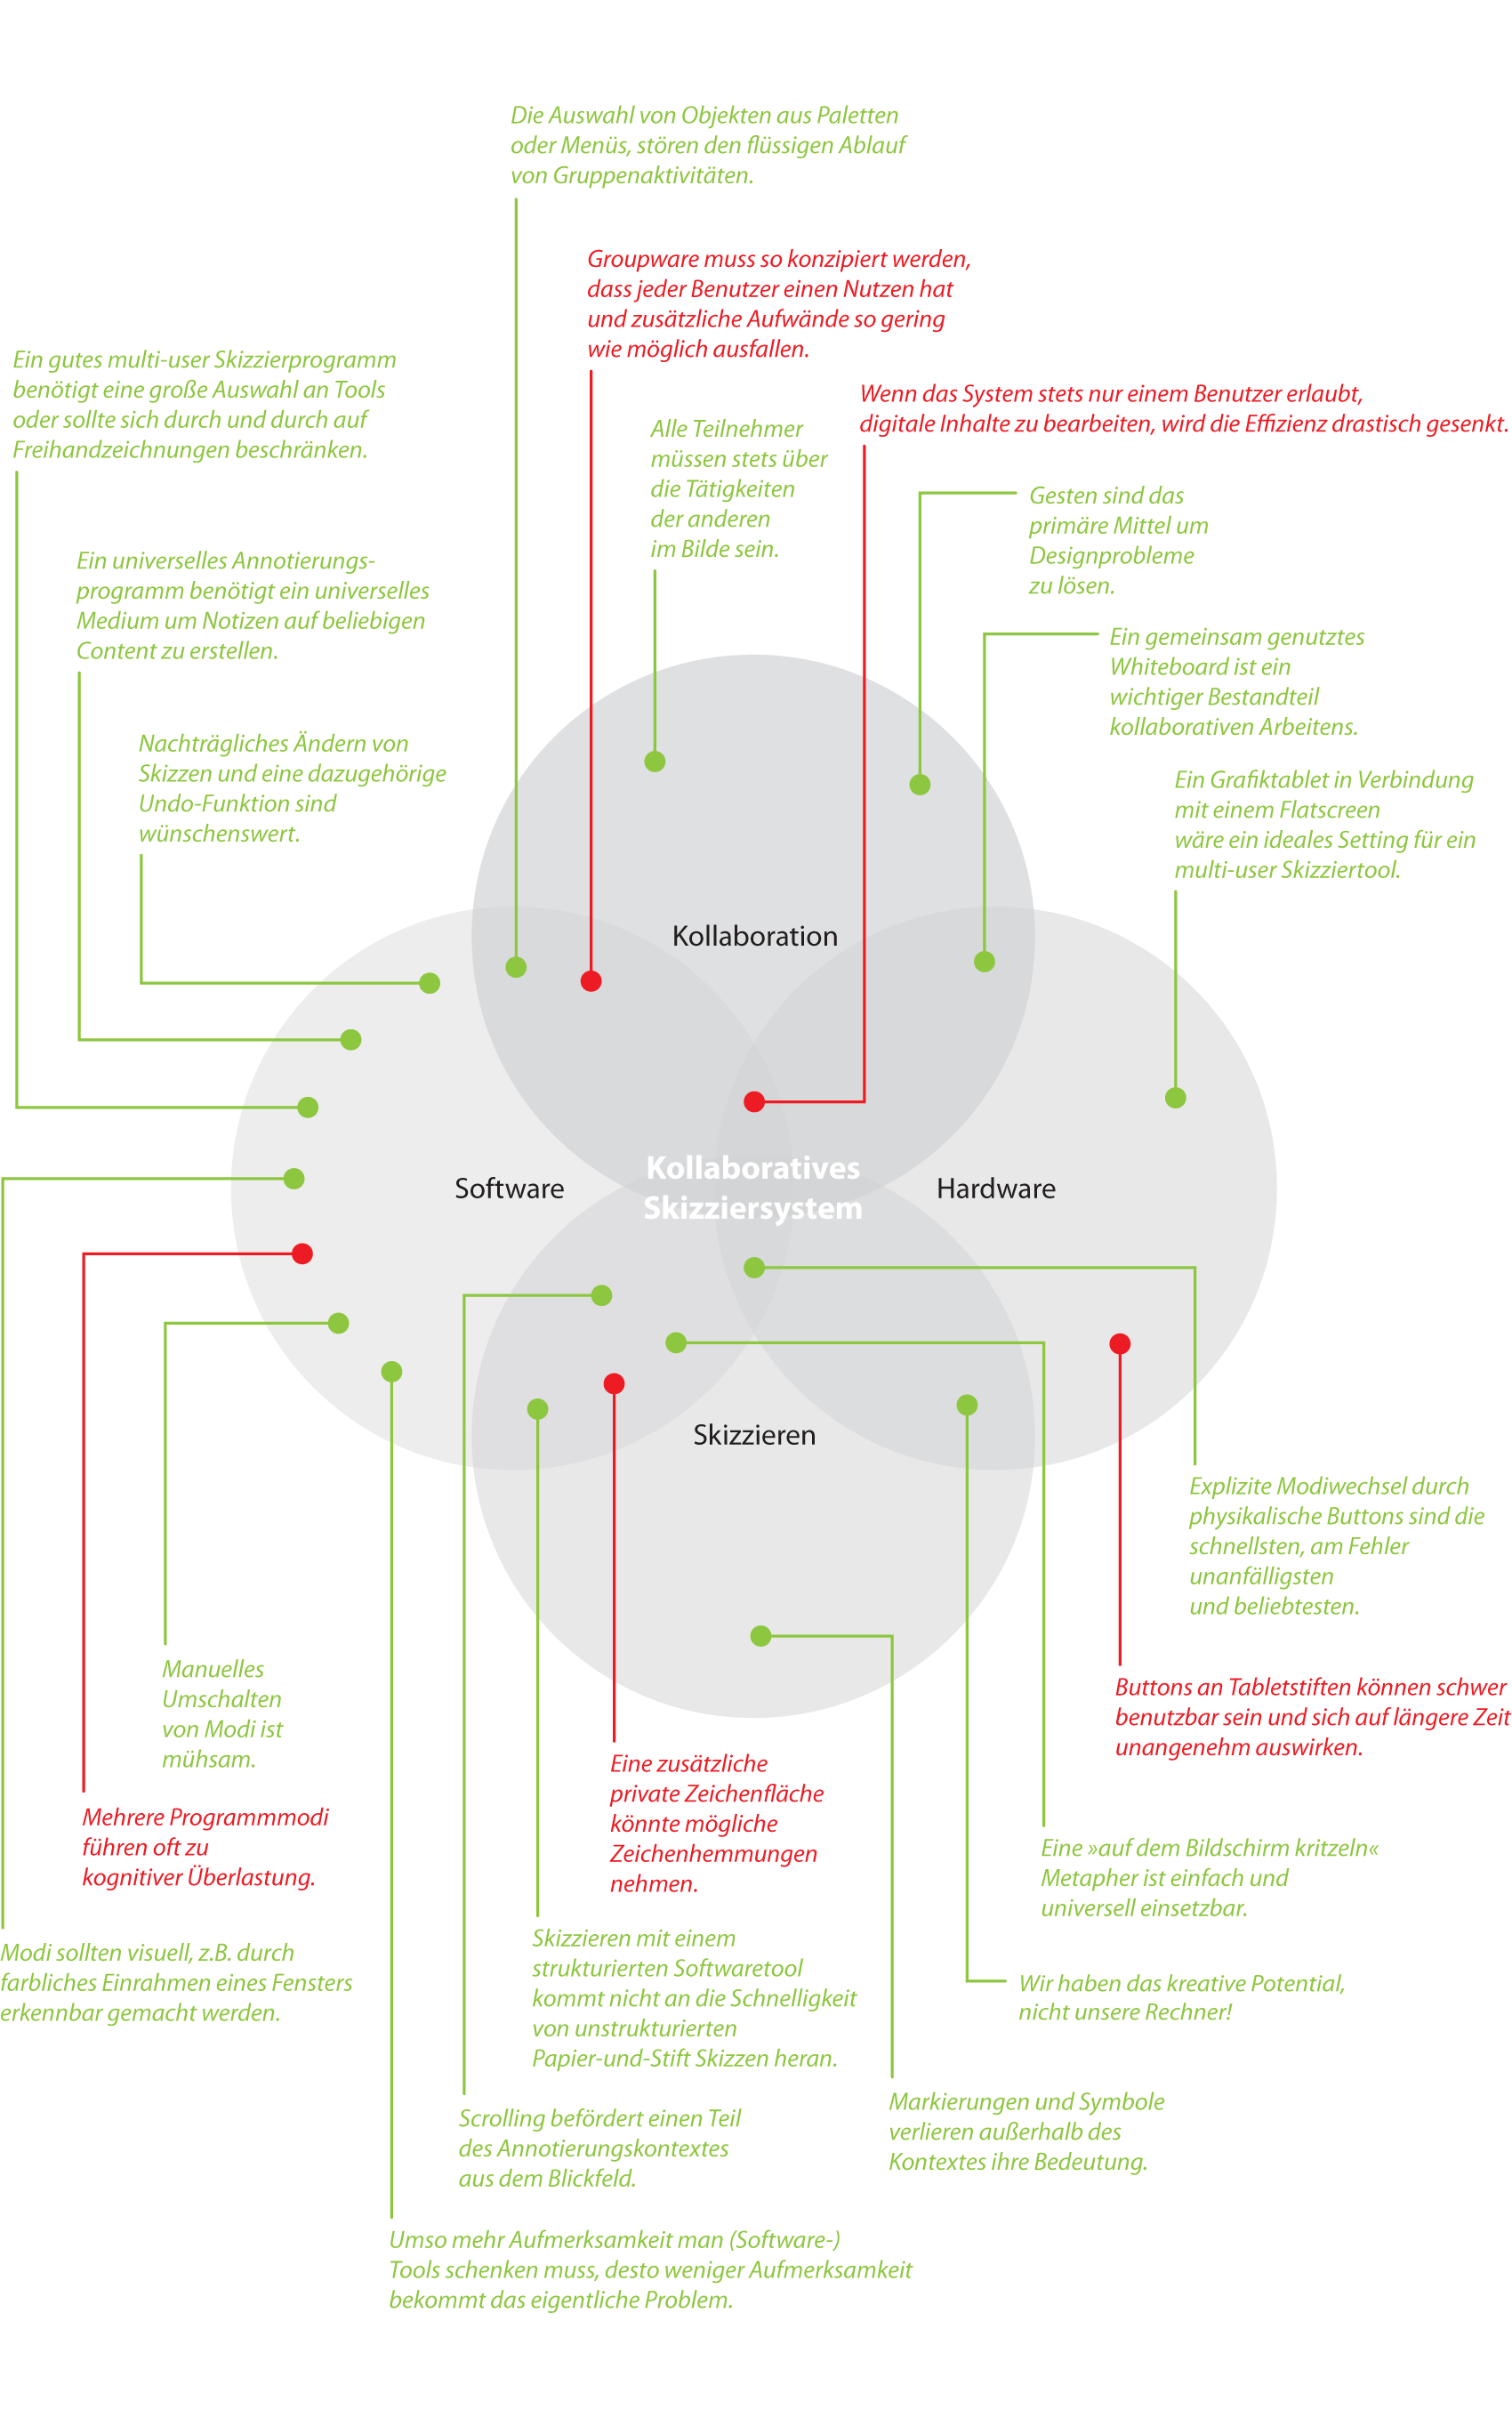
\includegraphics[bb=2cm 0cm 14.39cm 23.01cm]{gfx/scribblerAnforderungsauswertung}}
		\caption[Anforderungsauswertung für Scribbler]{Anforderungsauswertung für Scribbler. Alle umgesetzten Anforderungen sind in Grün gehalten. (Noch) nicht umgesetzte Anforderungen sind rot markiert.}\label{fig:scribblerAnforderungsauswertung}
\end{figure}

\subsubsection*{Software}
\scribbler sollte so simpel wie möglich aufgebaut sein und verzichtet auf einen großen Funktionsumfang. Daher beschränkt es sich auf einfache Freihandzeichnungen. So soll sichergestellt sein, dass die Aufmerksamkeit bei der Benutzung auf das Designproblem an sich und nicht auf das System selbst gerichtet wird. 

Durch die \emph{Accessibility} Funktion von \emph{Mac OS X} (vgl. \pointref{sec:programmLogik}) konnte \scribbler zu einem universellen Medium werden, das ermöglicht, auf beliebigen Content zu zeichnen. Es konnte ein Annotierungsprogramm entwickelt werden, das es in dieser Form noch nie zuvor gegeben hat. 

Das Umschalten der Modi kann wie vorher beschrieben explizit durch Tabletbuttons geschehen, oder auch implizit durch das Wechseln zwischen der Maus und einem Tabletstift. Die implizite Methode verursachte keine Probleme. Für den expliziten Wechsel wurde die Kennzeichnung des Modus durch eine farbliche Fensterumrandung eingeführt. Da die Umrandung aber erst erschien, wenn ein Stift in der Nähe des Tablets war, kam es trotzdem zu Verwirrungen. 

Schlussendlich bietet \scribbler eine Undofunktion die sich im Gegensatz zur Radierfunktion als äußerst hilfreich herausstellte.

\subsubsection*{Kollaboration} 
Durch die hardwarespezifischen Einschränkungen war es unmöglich, die Bedürfnisse aller Benutzer abzudecken. Die Koordinationsaufwände stiegen dadurch ebenfalls. Aus diesem Grund war es aber stets klar, wer gerade auf einem digitalen Artefakt zeichnet. Folglich waren alle über die Tätigkeiten der anderen im Bilde.

Durch das Fehlen unnötiger Paletten oder Menüs konnte ebenfalls ein flüssigerer Ablauf von Aktivitäten gesichert werden. Da sich alle Mitglieder der jeweiligen Testsessions im selben Raum aufhielten und durchgehend Sichtkontakt behielten, waren Gesten fortwährend vorhanden und konnten so zur Lösung eines Problems beitragen.

\subsubsection*{Skizzieren} 
\scribbler ist ein unstrukturiertes Skizzier- und Annotationstool. Durch die Verbindung mit den Grafiktablets kommt es durchaus an die Schnelligkeit von Papier-und-Stift Skizzen heran. Während der Laufzeit von \scribbler wird stets der Kontext zu den Skizzen bewahrt. Somit stellt Scrolling auch kein Problem dar. 

Gerade die Tests am Beginners' Day zeigten, dass durchaus Hemmungen beim Erstellen von Zeichnungen auftreten. Private Zeichenflächen könnten dagegen helfen, fehlen derzeit aber noch im Prototypen.

\clearpage

\section*{Zusammenfassung}
Die umfangreiche wissenschaftliche Recherche enthüllte viele verschiedene Systeme, die als Inspiration und Wegweiser für die Entwicklung von \scribbler dienten. Durch die Erfahrungen, die Wissenschaftler in der Vergangenheit gemacht haben, konnte ein klares Anforderungsprofil an kollaborative Skizzier- und Annotationssoftware geschaffen werden. \scribbler wurde mit dieser Prämisse vor Augen entwickelt. Es handelt sich dabei um ein technisches System, das Menschen in kollaborativen Meetings beim Skizzieren und Annotieren unterstützen soll. Am sinnvollsten kann \scribbler von Designern, zur Optimierung des Designprozesses, oder von Lehrenden, zur besseren Veranschaulichung von Lehrinhalten, genutzt werden. \scribbler unterscheidet sich insofern von anderen Systemen, als dass es eine semantische Verknüpfung zwischen Drittapplikationen und ihnen zugehörigen Zeichnungen, bzw. Skizzen schafft. Das Gezeichnete haftet am darunter liegenden Programmfenster und sogar an darin befindlichen Inhalten, wie beispielsweise Webseiten. Daher kann damit ganz anders gearbeitet werden, als mit Systemen, die einfach ein statisches Bild über darunter liegende Fenster legen. \scribbler verfügt über einen innovativen Charakter und bietet Funktionen, die es zuvor in dieser Form noch nicht gegeben hat. Dies gebührt nicht zuletzt dem aktuellsten Mac Betriebssystem OS X 10.6, das zum ersten mal Entwicklern die dafür notwendigen Funktionen zur Verfügung stellt. Neben diesen positiven Eigenschaften gibt es auch einige Nachteile, beispielsweise das teure und umfangreiche Hardware-Setting oder das Fehlen umfangreicher Zeichenoptionen, das es für den Einsatz als komplexes Skizziertool unbrauchbar macht. Das Projekt \scribbler hat den aktuellen Stand von Technik und Wissenschaft genutzt und ein neuartiges System entwickelt, das im Gegenzug neue Eigenheiten und Aspekte hervorgebracht hat, die bei einer Weiterentwicklung in Betracht gezogen werden müssen. 
